
\subsection{Studies in the General Phase Space} % (fold)
\label{sub:coarse_studies}

In order to examine the overall discrimination performance of the DNN's to that of the physics-driven variables, we examine the ROC curves in Figure~\ref{fig:combinedROC1}. In particular, we compare the DNN's to $n$-subjettiness~\cite{nsub} $\tau_{21} = \tau_{2}/\tau_{1}$, the jet mass, and the distance $\Delta R$ between the leading two $p_{T}$ subjets.  In Figure~\ref{fig:combinedROC1a}, we can see that the three DNN's have similar performance, but the MaxOut networks tends to outperform the ConvNet networks.  We suspect that the MaxOut tends to outperform the ConvNets due to sparsity of the jet-images, whereby the MaxOut network views the full jet-image from the inital hidden layer while the sparsity tends to make it difficult for the ConvNets to learn meaningful convolution filters .  We also see that the ConvNet-Norm tends to outperform the ConvNet trained on the un-normalized jet-images.  As we will see soon,  it is difficult for these networks to fully learn the jet mass and thus the loss of mass information from normalization and energy  binning (rather than transverse energy) of the ConvNet-Norm training tends to not to impede performance.   Finally, we can see the Fisher-Jet discriminant\footnote{The Fisher discriminant is trained in three partitions of $\Delta  R$ ($\Delta R \in [0.25, 0.5],\ [0.5, 0.75],\ [>0.75])$, in order to account for the non-linear variation in jet-images from the differing positions of the two subjets.} performance, as described in reference~\ref{JetImages}, which outperforms the physics inspired variables (as expected) but is much less performant than the DNN's. In addition, in Figure~\ref{fig:combinedROC1b} we see that the DNN's also outperform the two-variable combinations of the physics inspired variables (computed using the 2D likelihood ratio).   It is interesting to note that combining mass and $\tau_{21}$, or $\tau_{21}$ and $\Delta R$, achieve much higher performance than the individual variables and are significantly closer to the performance of the DNN's.
%This is likely due to the normalization and energy binning helping to provide more uniformity in the typical pixel intensities across jet-images.
\begin{figure}[!htbp]
\begin{center}
\subfloat[]{
	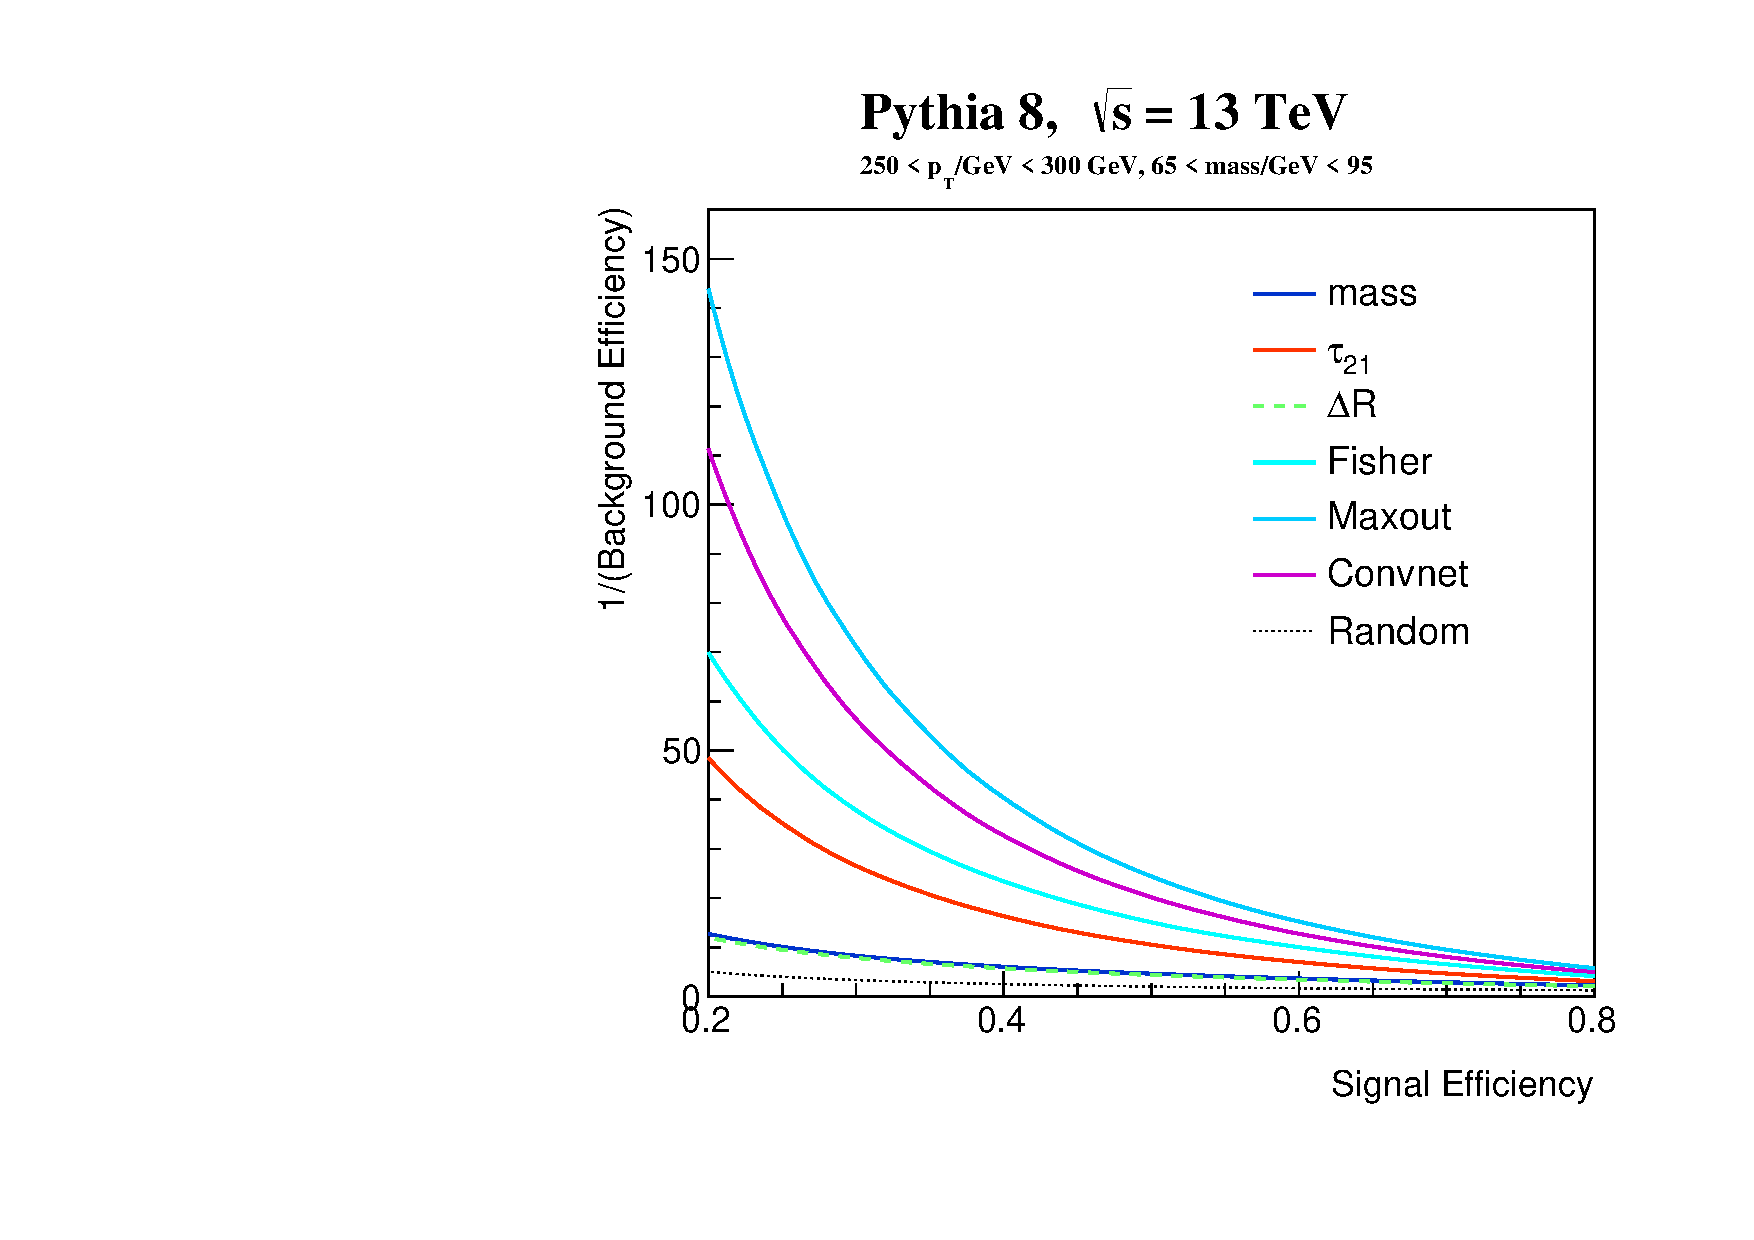
\includegraphics[width=0.48\textwidth,angle=0]{figures/ROC_1}
	\label{fig:combinedROC1a}
}
\subfloat[]{
	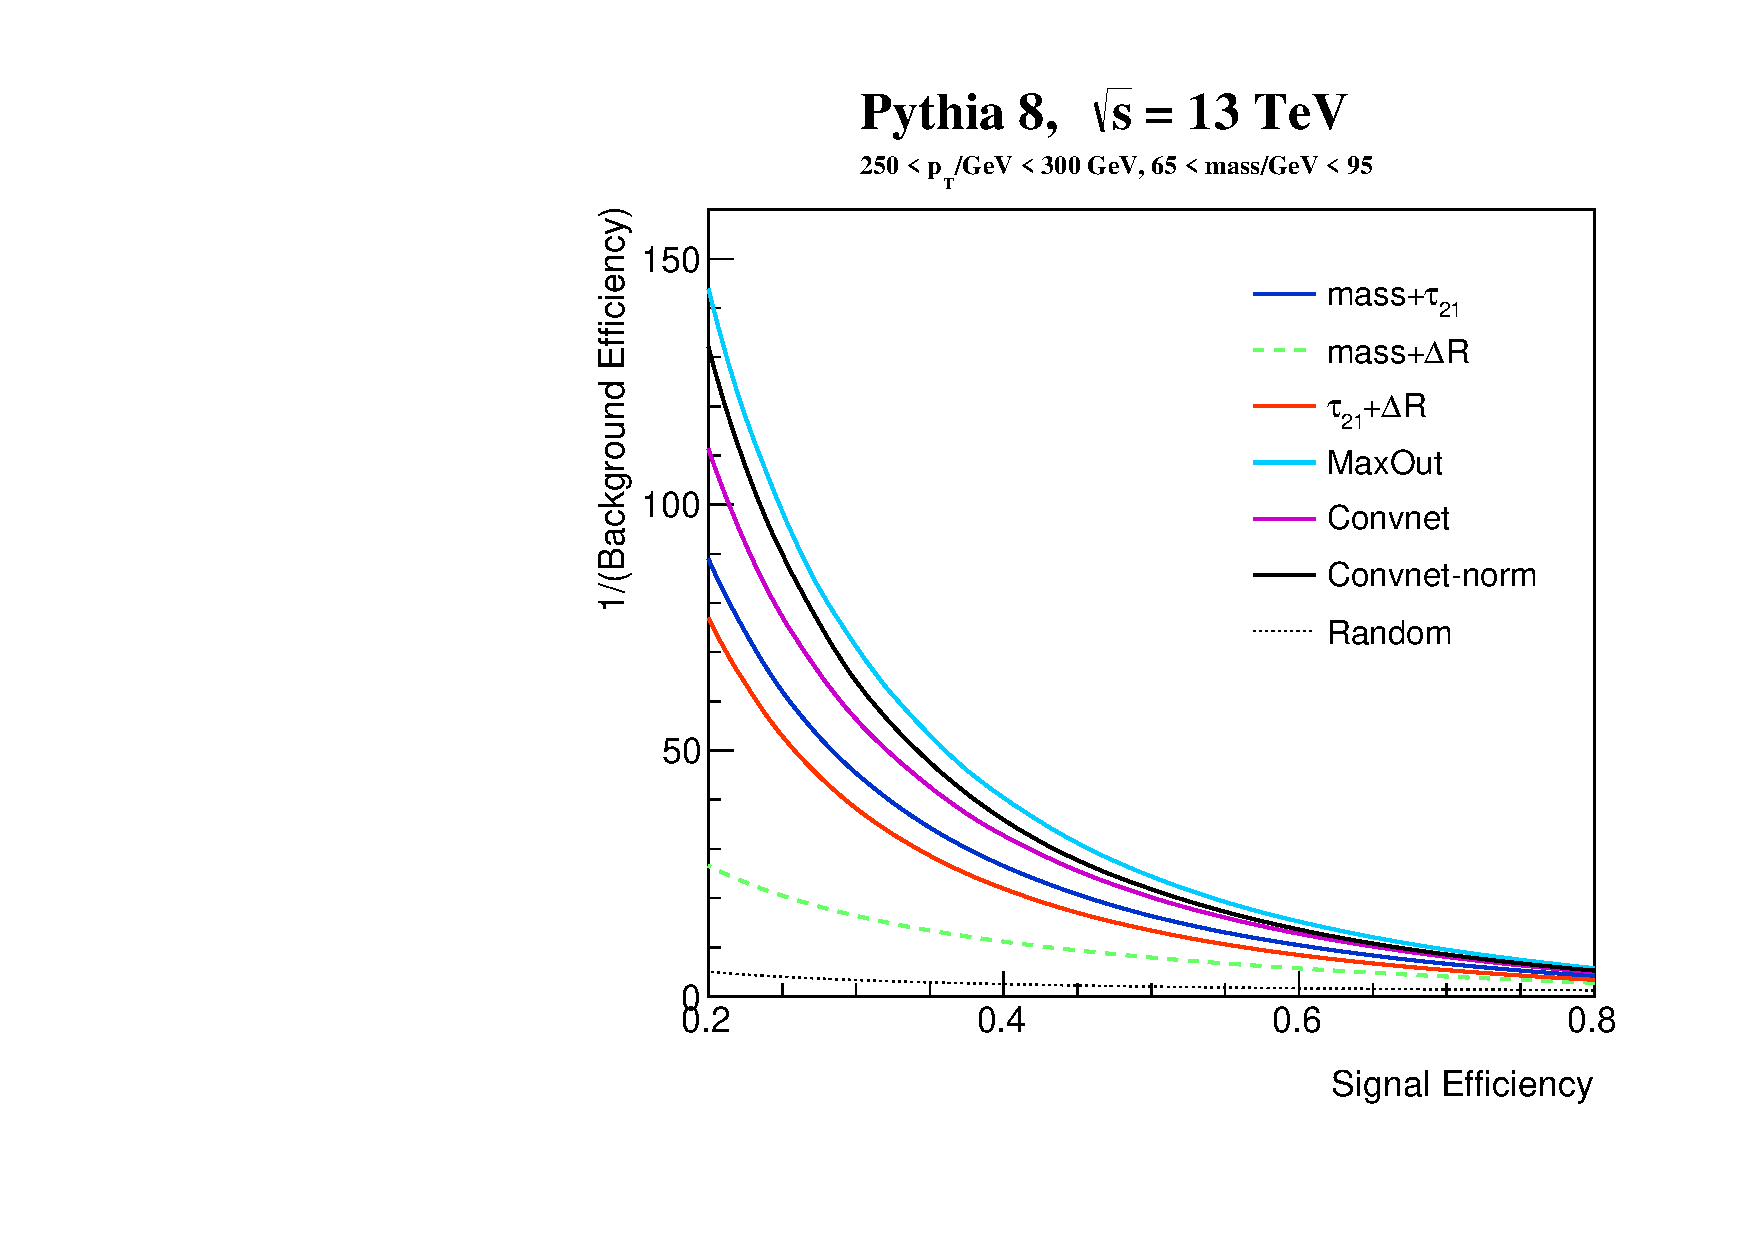
\includegraphics[width=0.48\textwidth,angle=0]{figures/ROC_2}
	\label{fig:combinedROC1b}
}
\end{center}
   \caption{Receiver Operating Characteristic (ROC) over coarse sample}
  \label{fig:combinedROC1}
\end{figure}





\begin{figure}[!htbp]
  \begin{center}
\subfloat[]{
	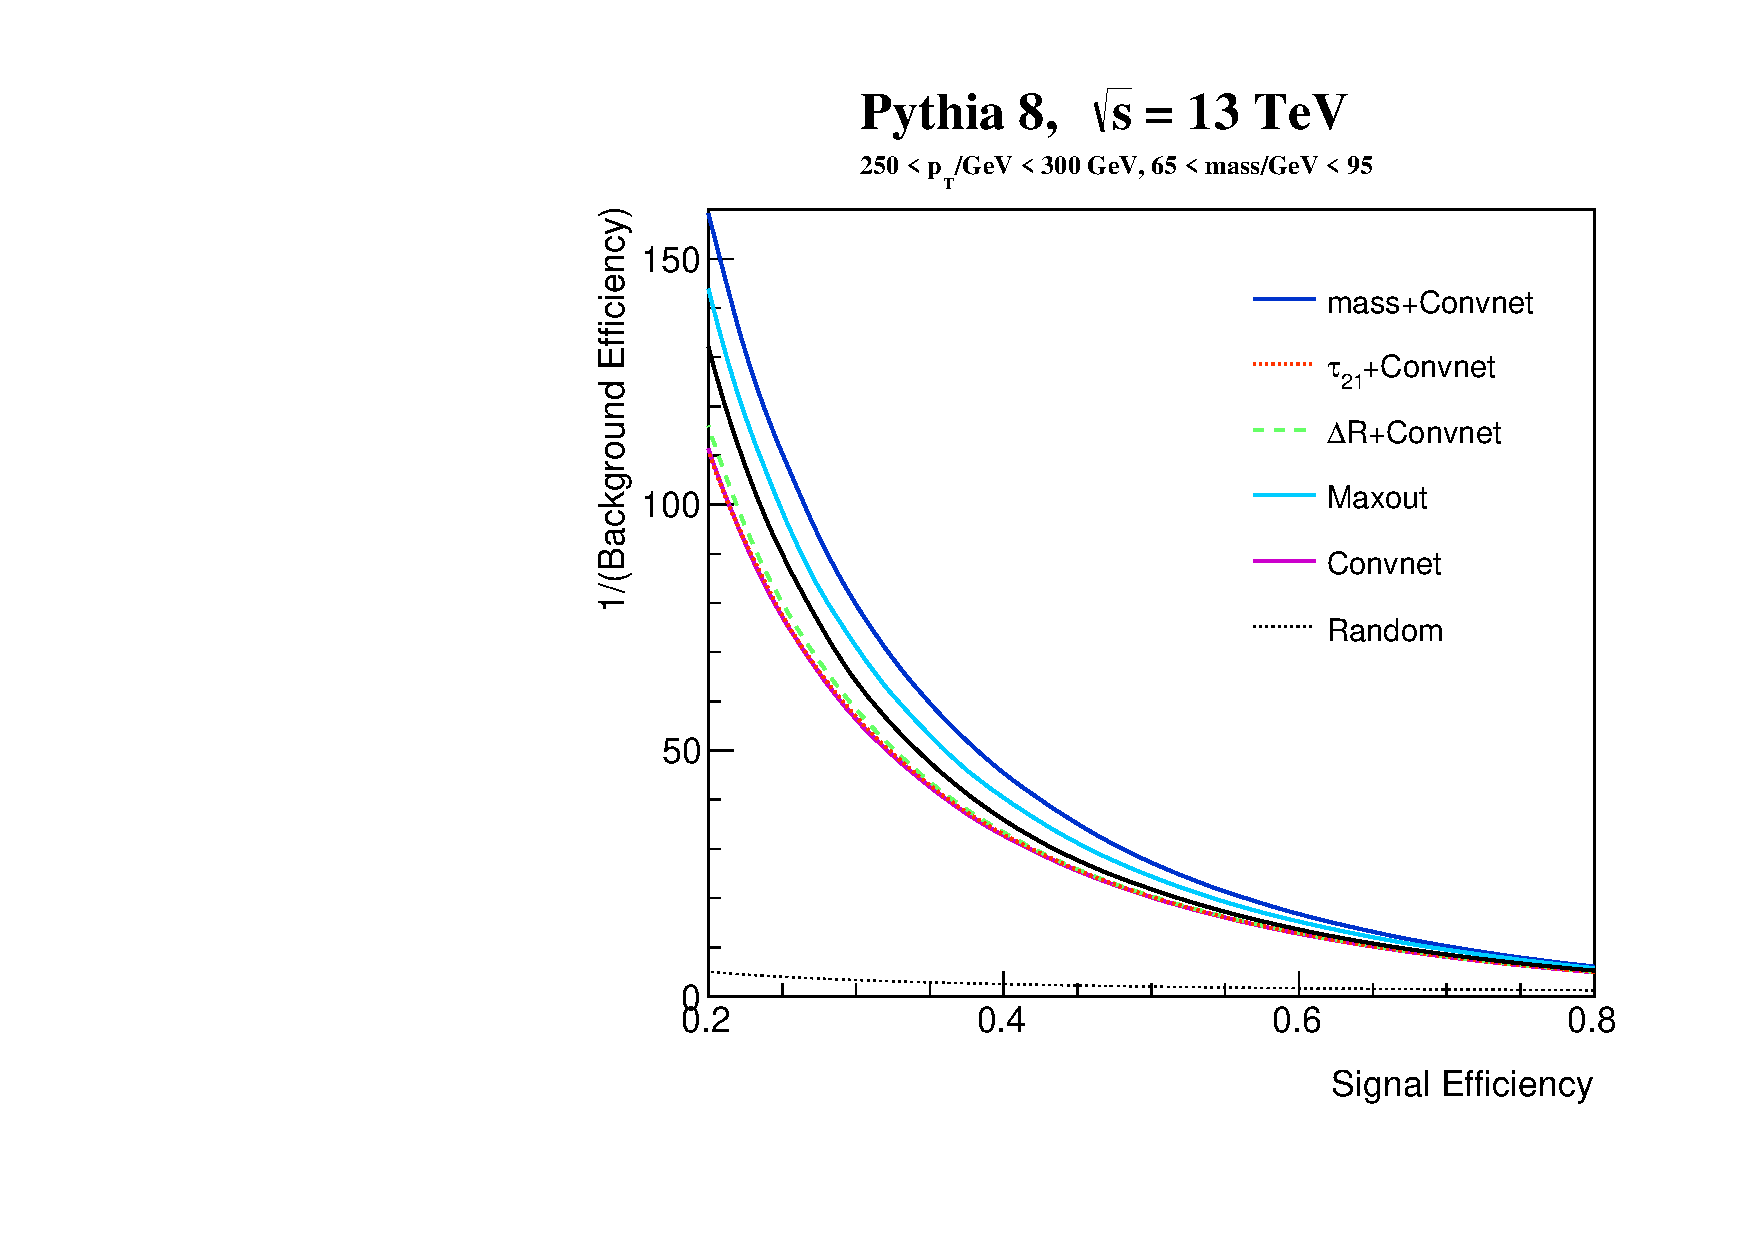
\includegraphics[width=0.48\textwidth,angle=0]{figures/ROC_3}
	\label{fig:combinedROC2a}
}
\subfloat[]{
	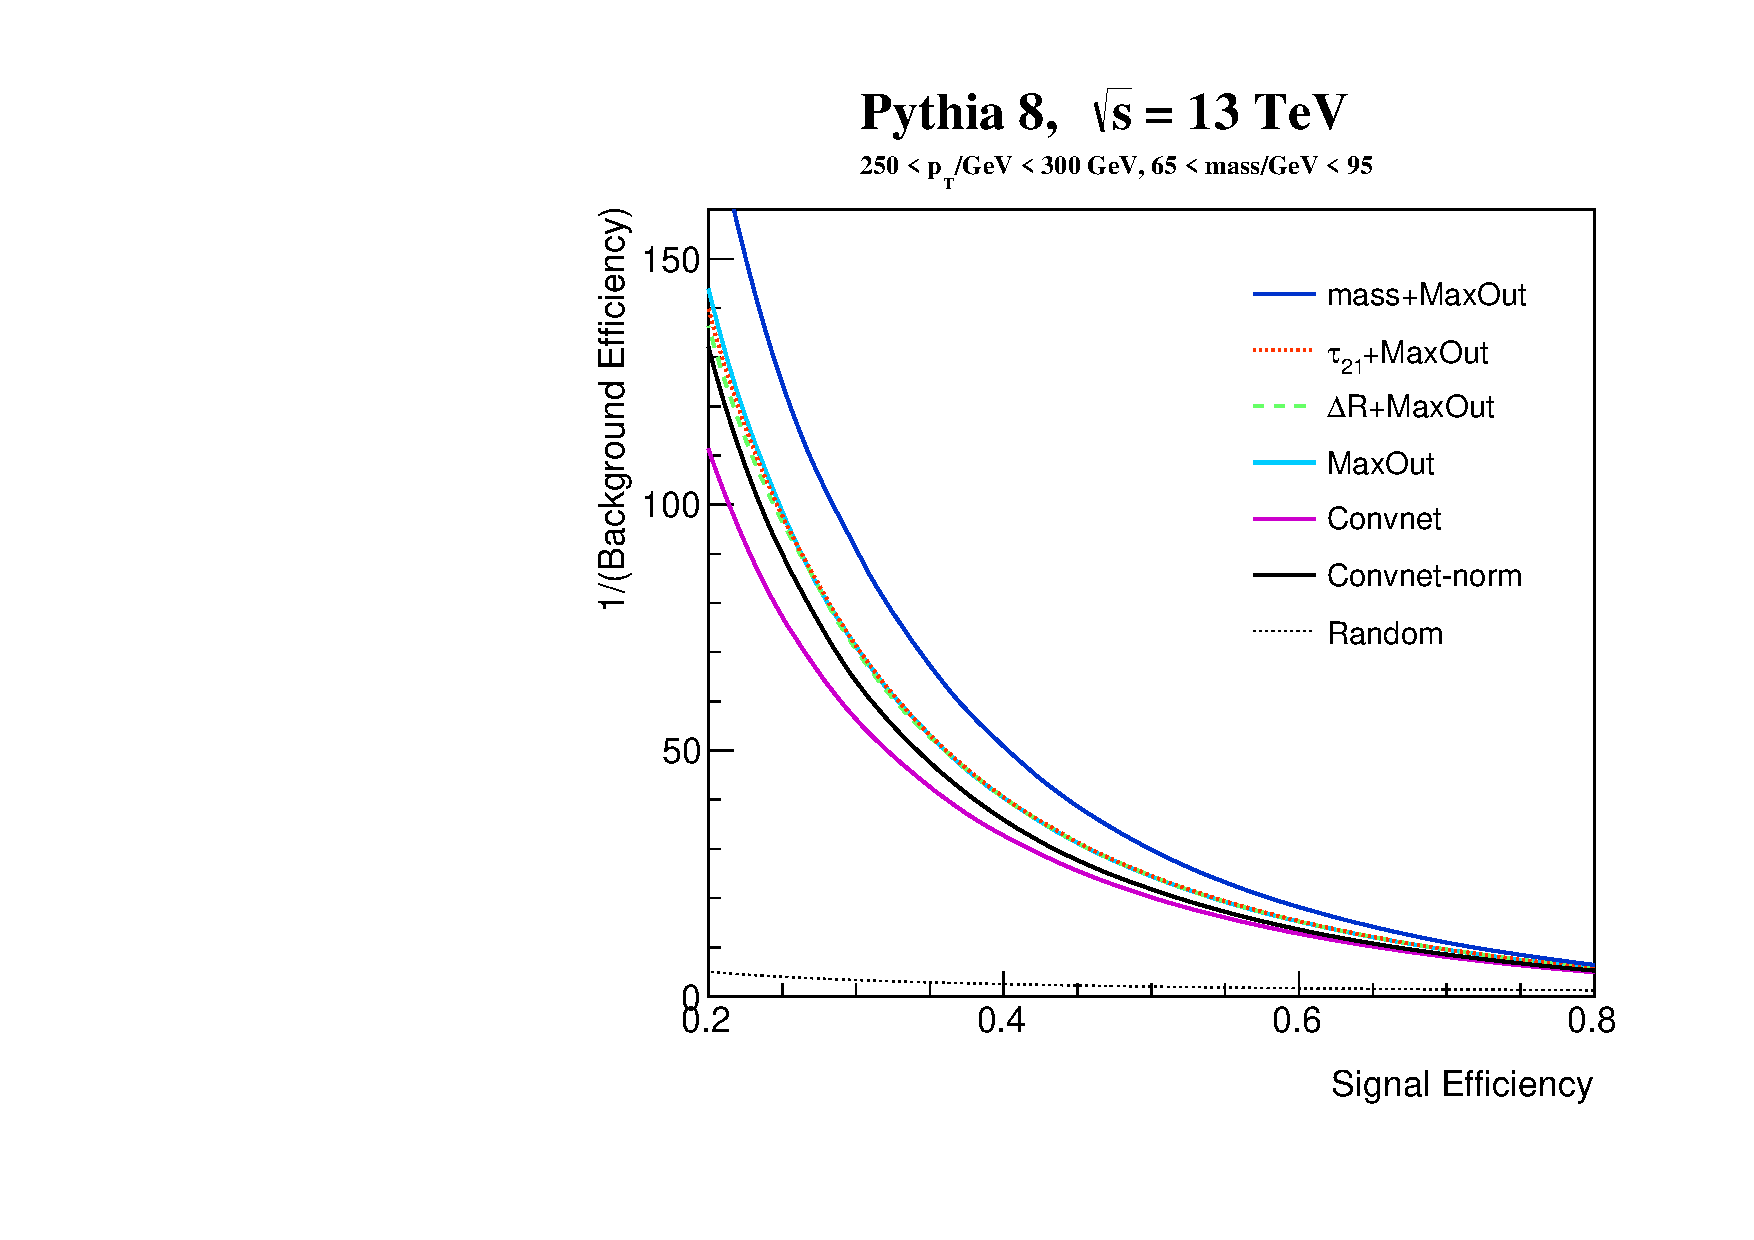
\includegraphics[width=0.48\textwidth,angle=0]{figures/ROC_4}
	\label{fig:combinedROC2b}
}
\end{center}
  \caption{Receiver Operating Characteristic (ROC) over coarse sample}
  \label{fig:combinedROC2}
\end{figure}

We also provide a comparison to a 3D likelihood constructed on $\tau_{21}$, jet mass, and the deep network output itself. We can gain a significant piece of insight from this. Note how in Figure~\ref{fig:combinedROC} we can see that the DNN represents a large gain on a physics-only likelihood. However, when we explicitly include the physics variable in a 3D likelihood, we see a small but definitively non-zero performance gain. This implies that the performance boost \emph{by definition} is getting its gain from something that is not \emph{fully} encapsulated in $\tau_{21}$ and jet mass. 

Though important on it's own, this figure of merit does little to help drive understanding in the context of HEP. Such an increase begs further questions -- what is this gain, and where does it come from? Why is the DNN able to pick up on this?



\subsubsection{Understanding what is learned} % (fold)
\label{ssub:understanding_what_is_learned}

% subsubsection understanding_what_is_learned (end)
In Figure~\ref{fig:convkernels}, we first examine the $11\times11$ convolutional filters in the first layer and look for structure. In

In order to understand what we learn, we first take a look \emph{inside} the deep network, and visualize features learned during training.

\begin{figure}[bt]
  \begin{center}
      \subfloat[$(11\times11)$ convolutional kernels from first layer \label{subfig:filters}]{
        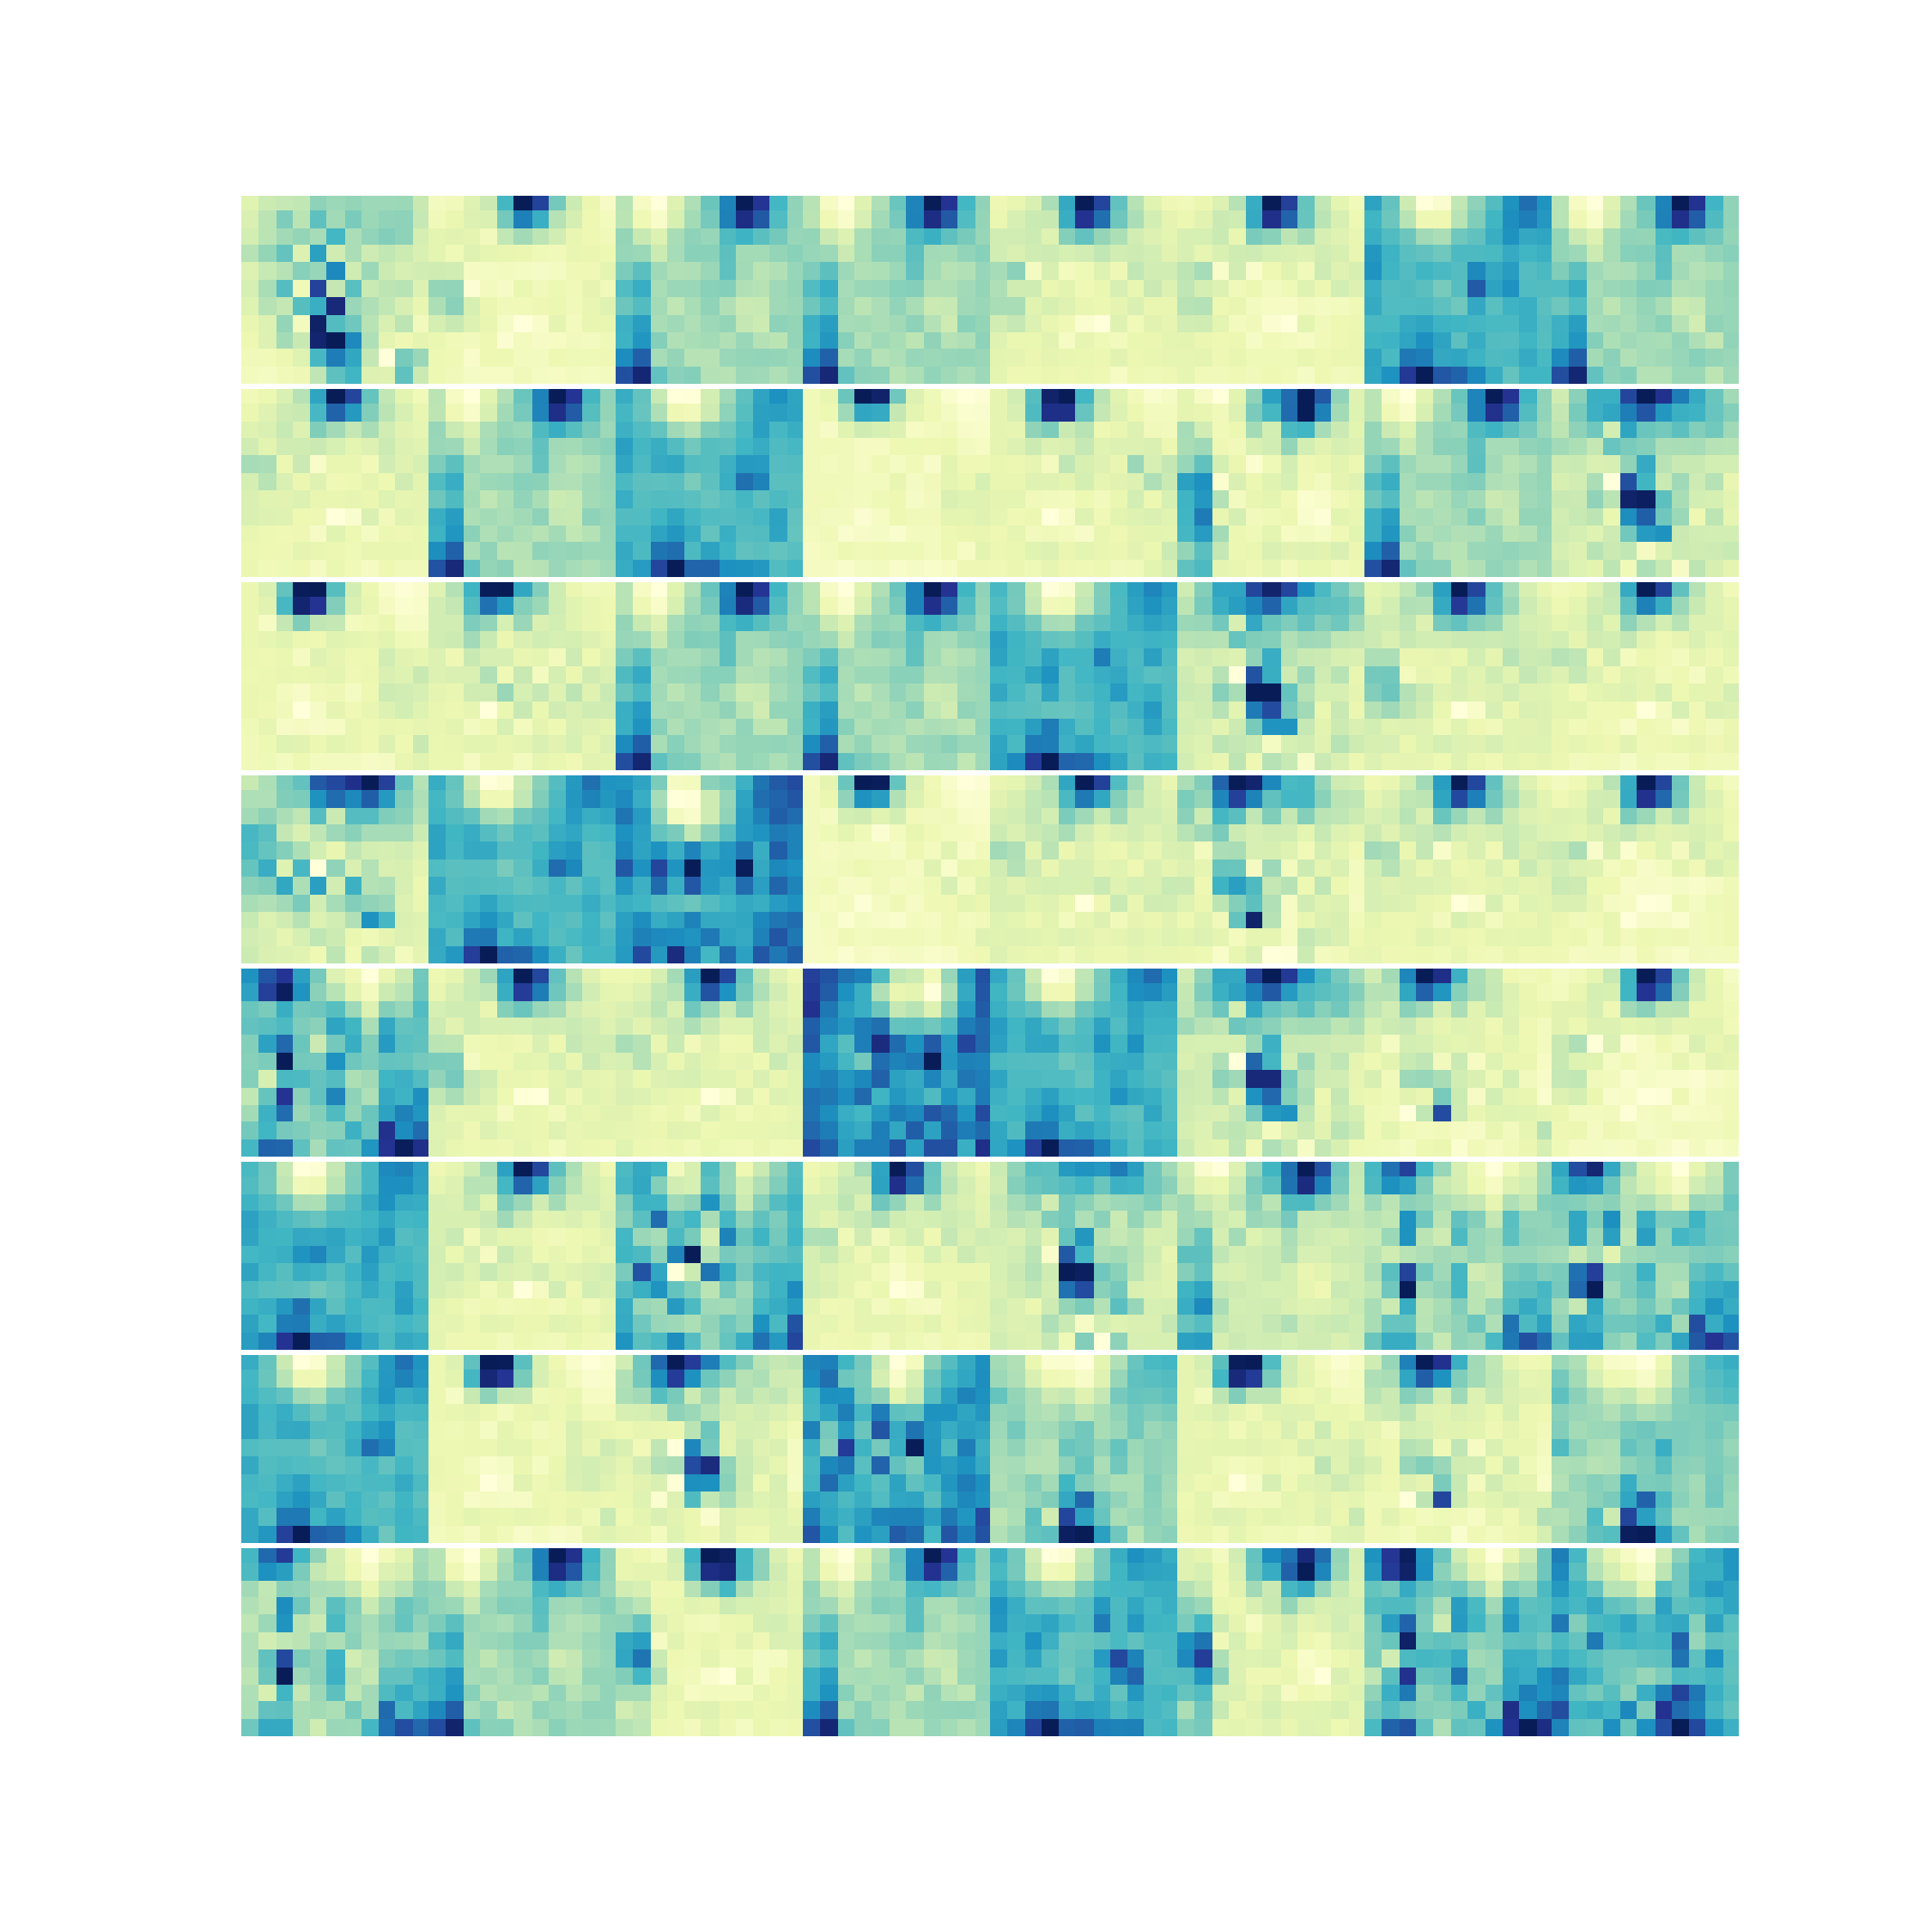
\includegraphics[width=0.5\textwidth]{figures/conv-filts.pdf}
      }
      \subfloat[Convolved Jet Image differences\label{subfig:convolvedfilters}]{
        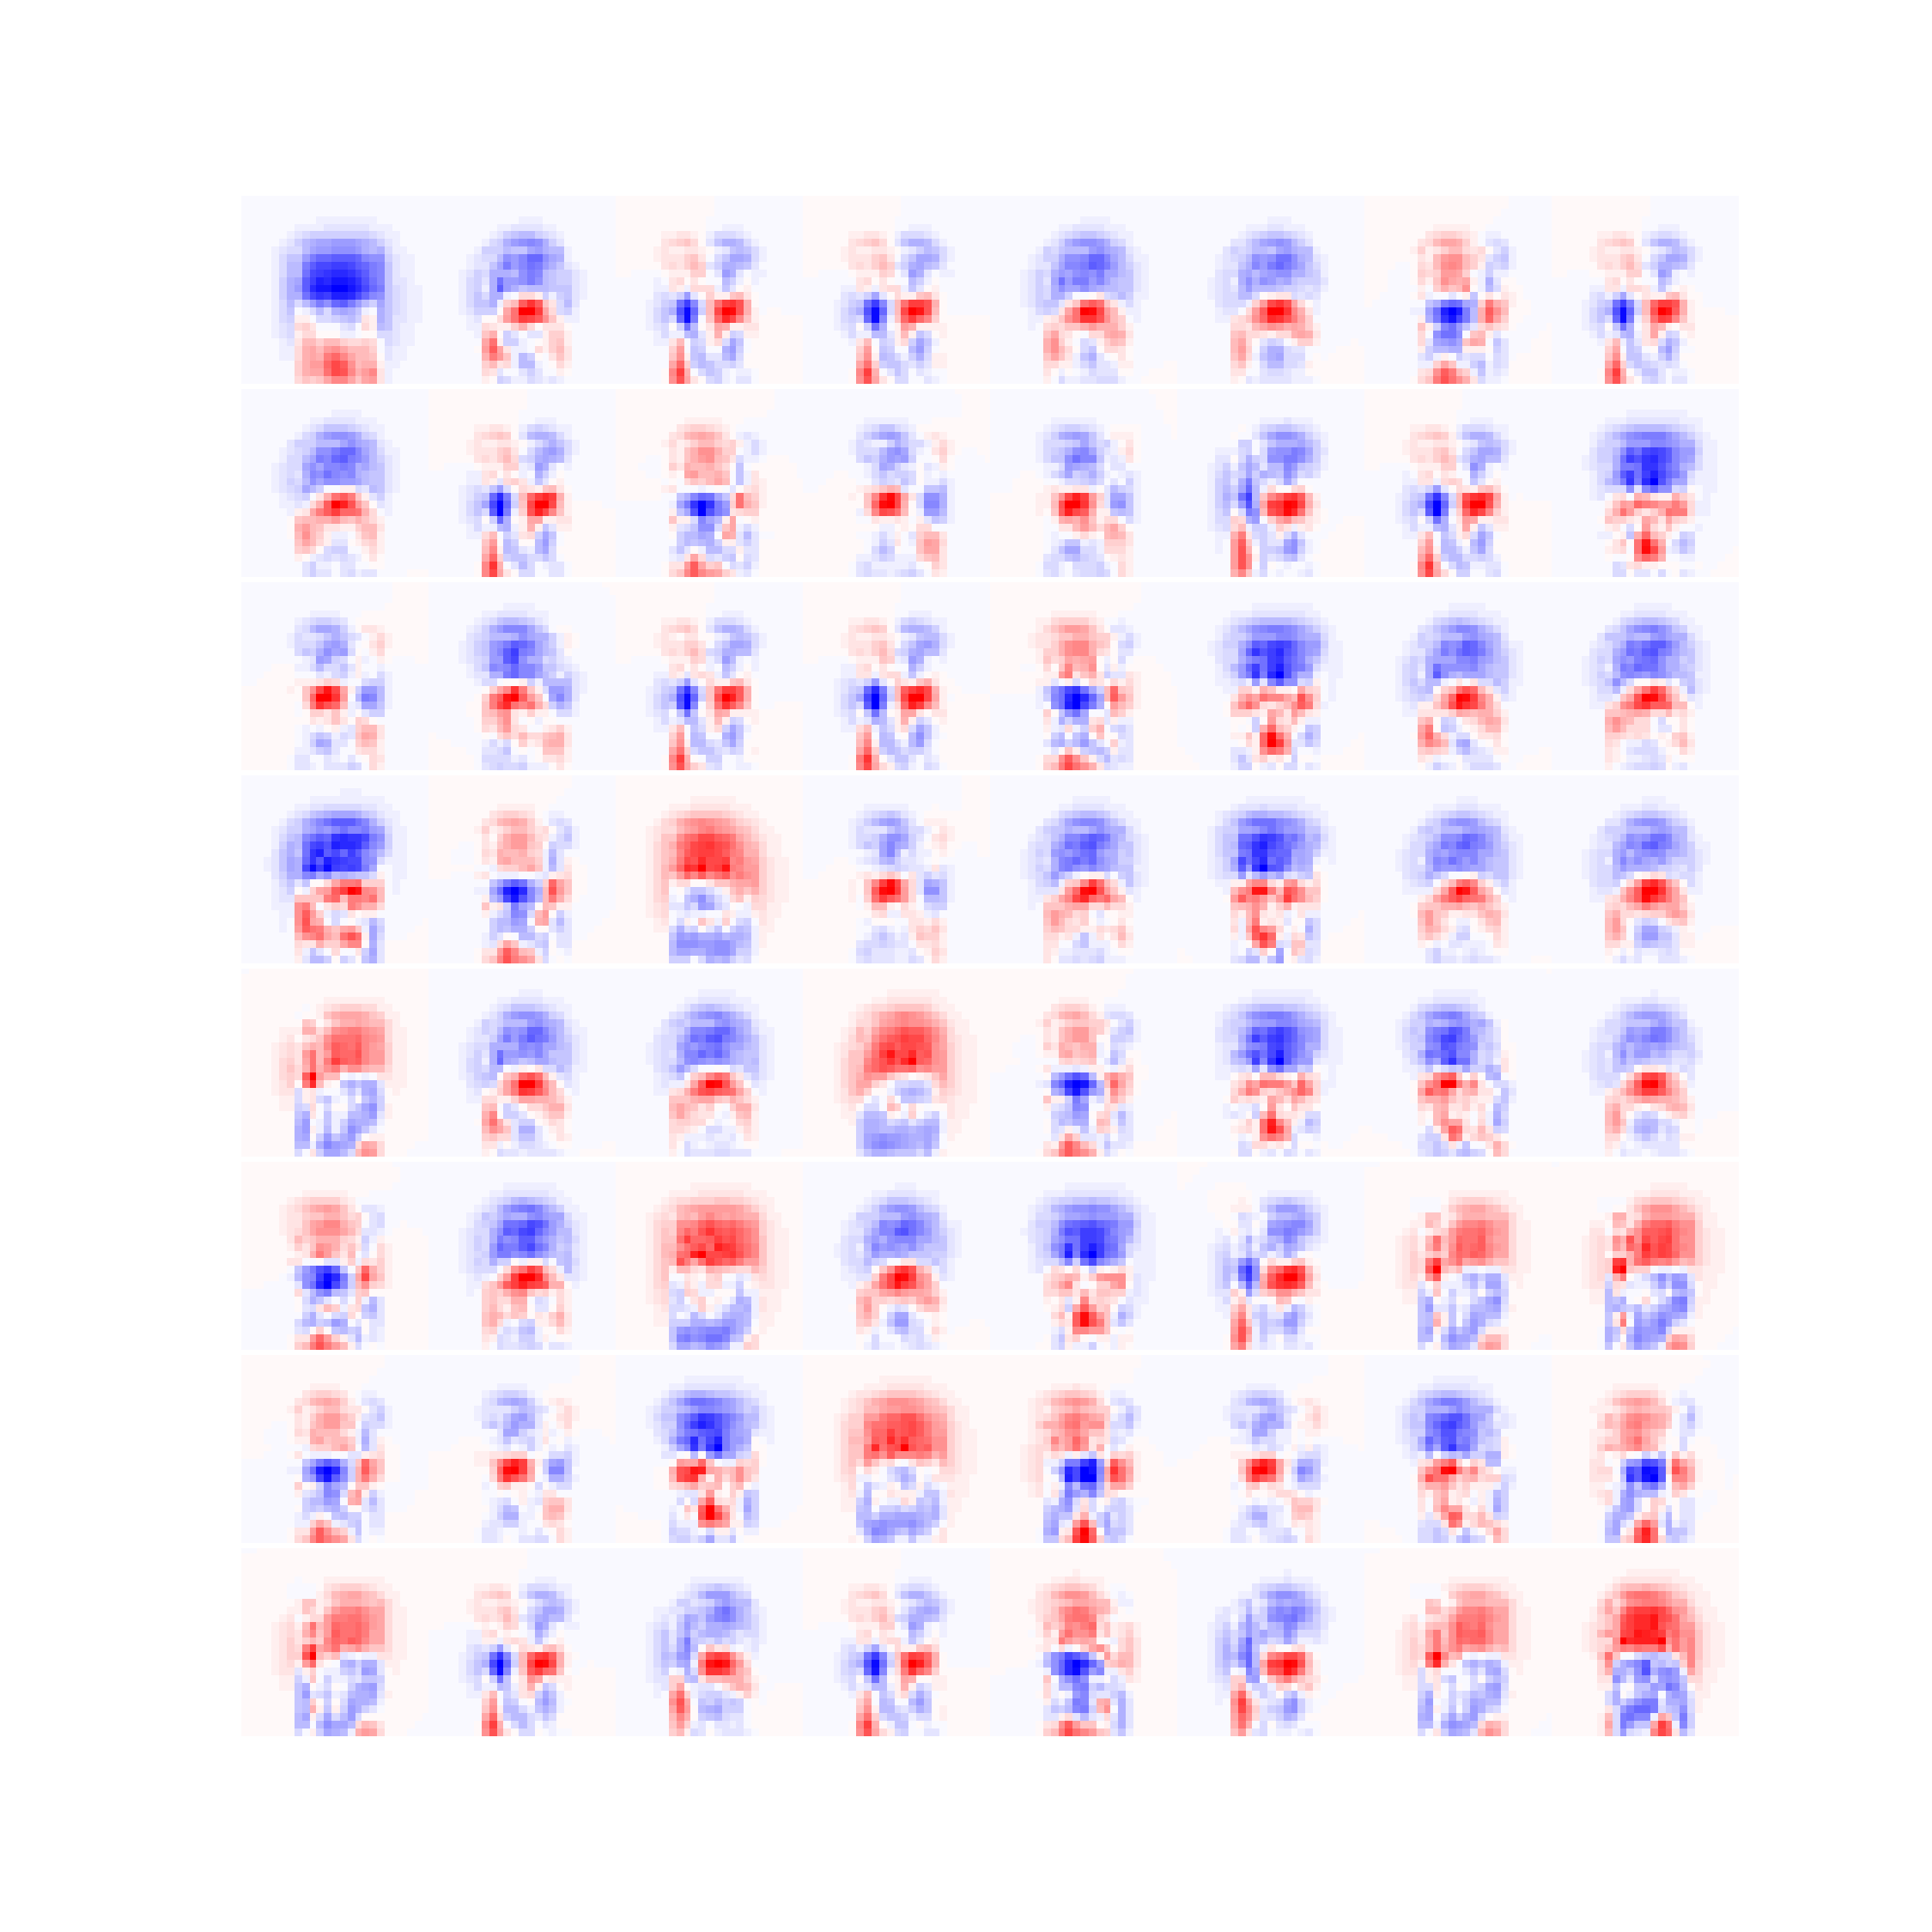
\includegraphics[width=0.5\textwidth]{figures/conv-diffs-global.pdf}
      }
      \caption{Convolutional Kernels (left), and convolved feature differences in jet images (right)}
      \label{fig:convkernels}

    \end{center}
\end{figure}

\begin{figure}[bt]
  \begin{center}
      \subfloat[Sculpted QCD $\Delta R$ distribution\label{fig:sculpteddR}]
      {
        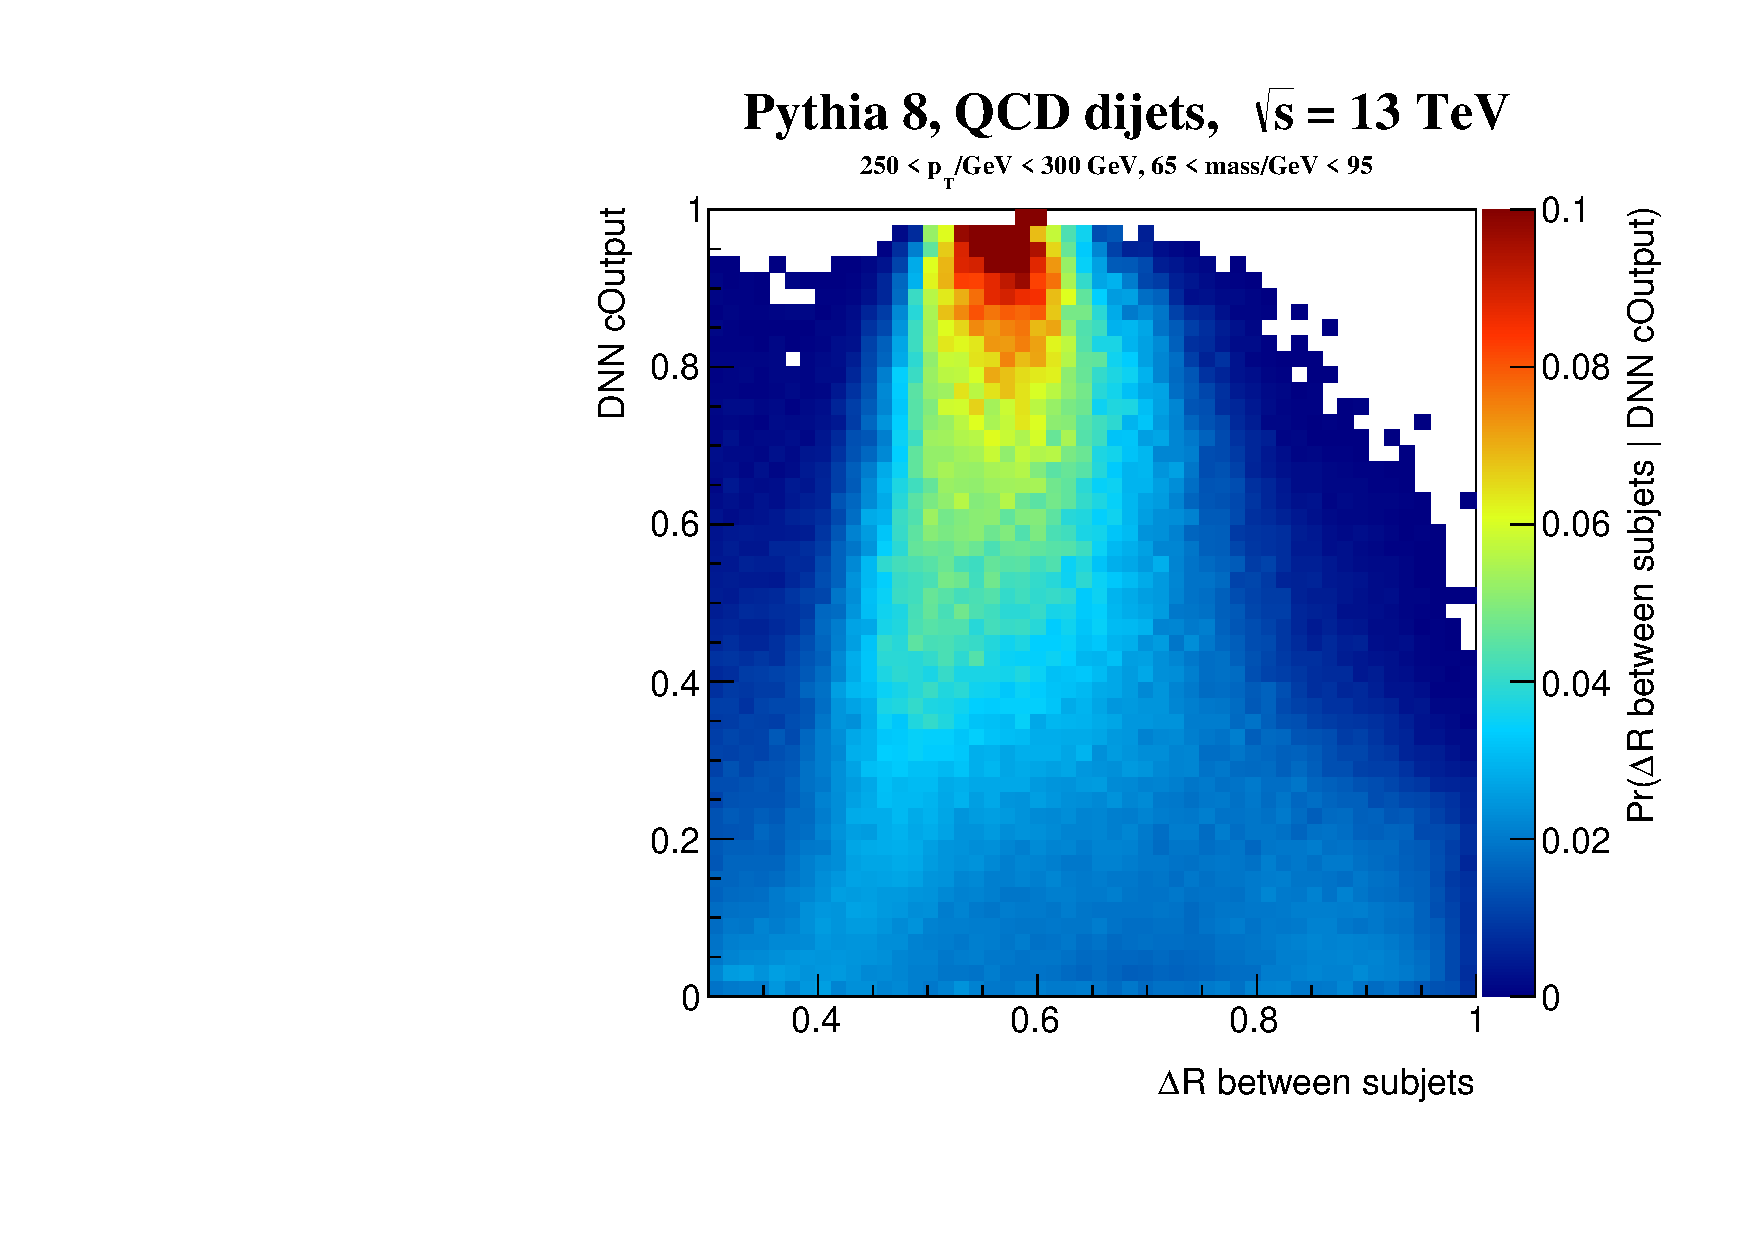
\includegraphics[width=0.45\textwidth]{figures/dR_convnet_back_norm_invert.pdf} 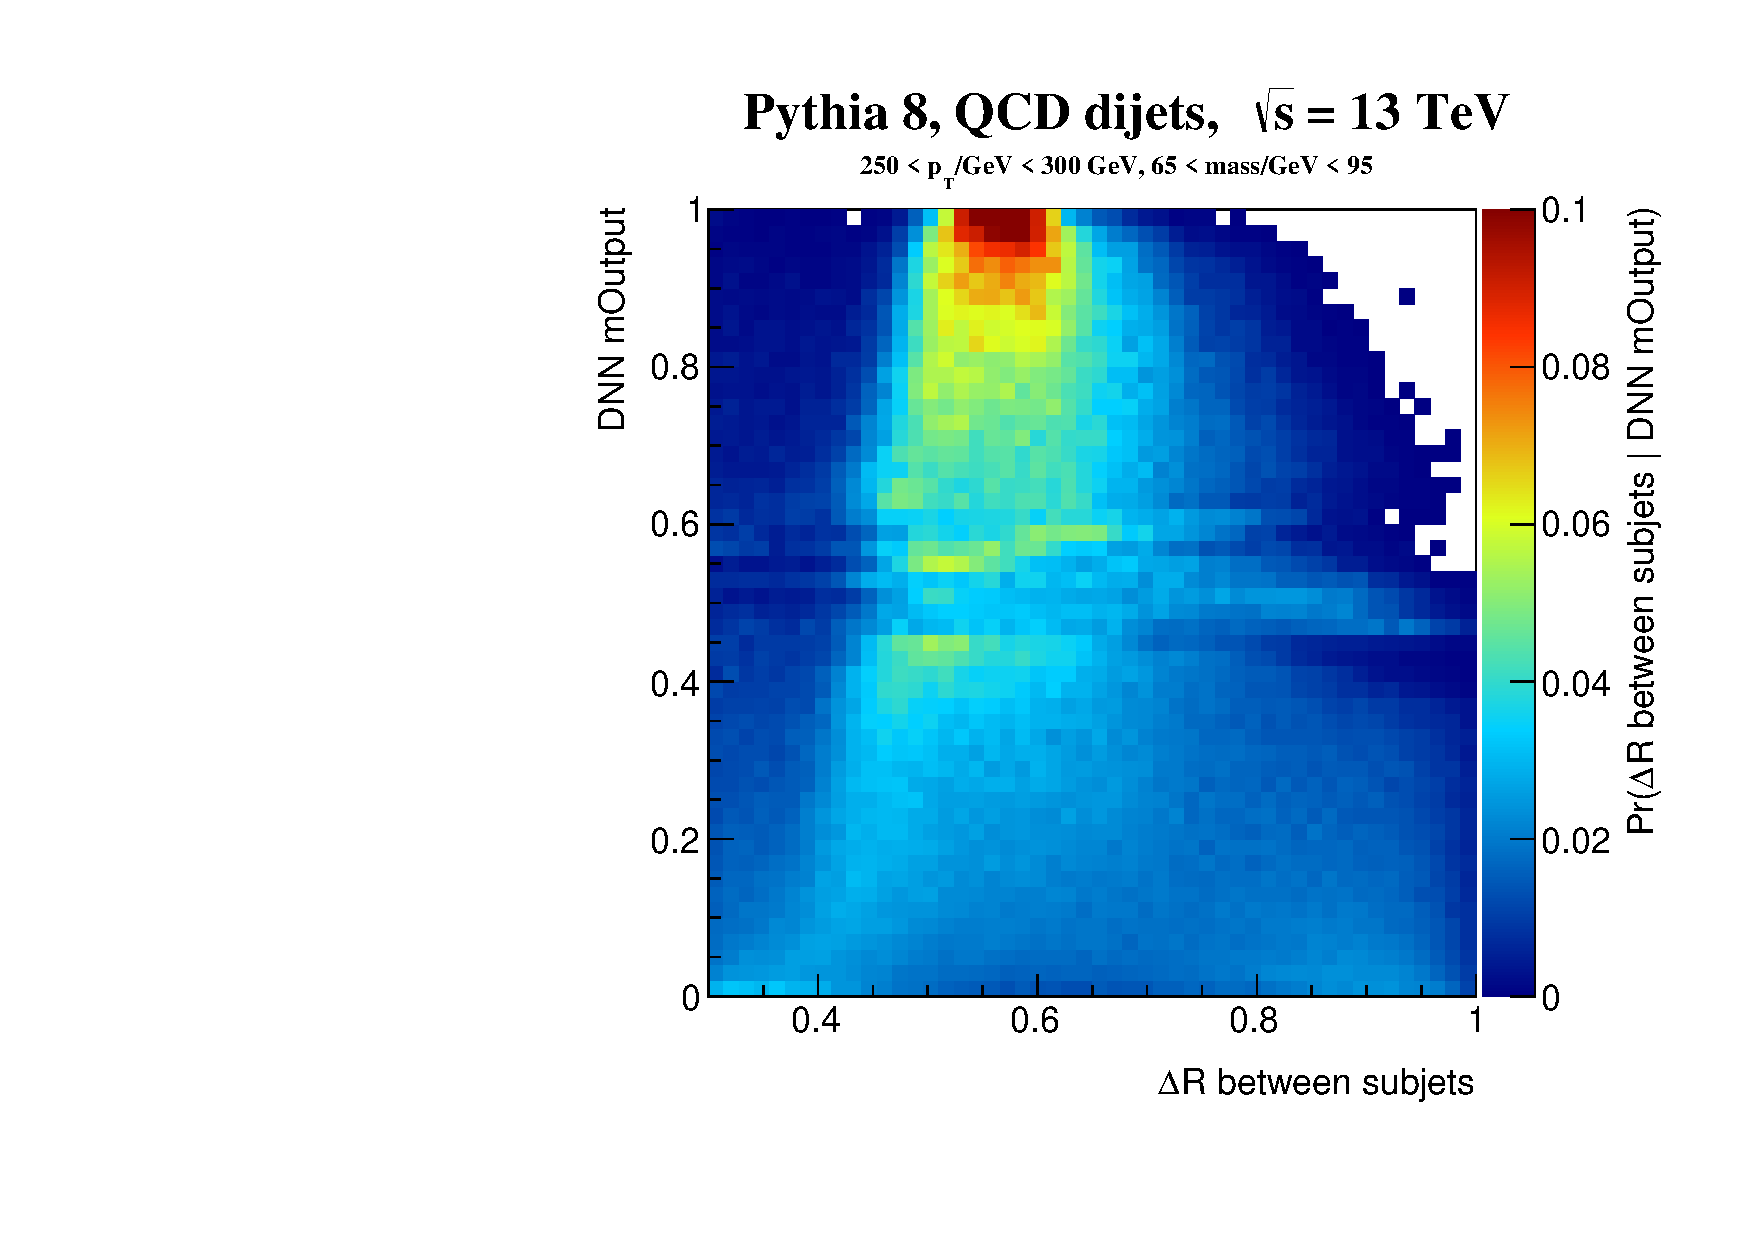
\includegraphics[width=0.45\textwidth]{figures/dR_maxout_back_norm_invert.pdf}
      }\\
      \subfloat[Sculpted QCD $\tau_{21}$ distribution\label{fig:sculptednsj}]
      {
        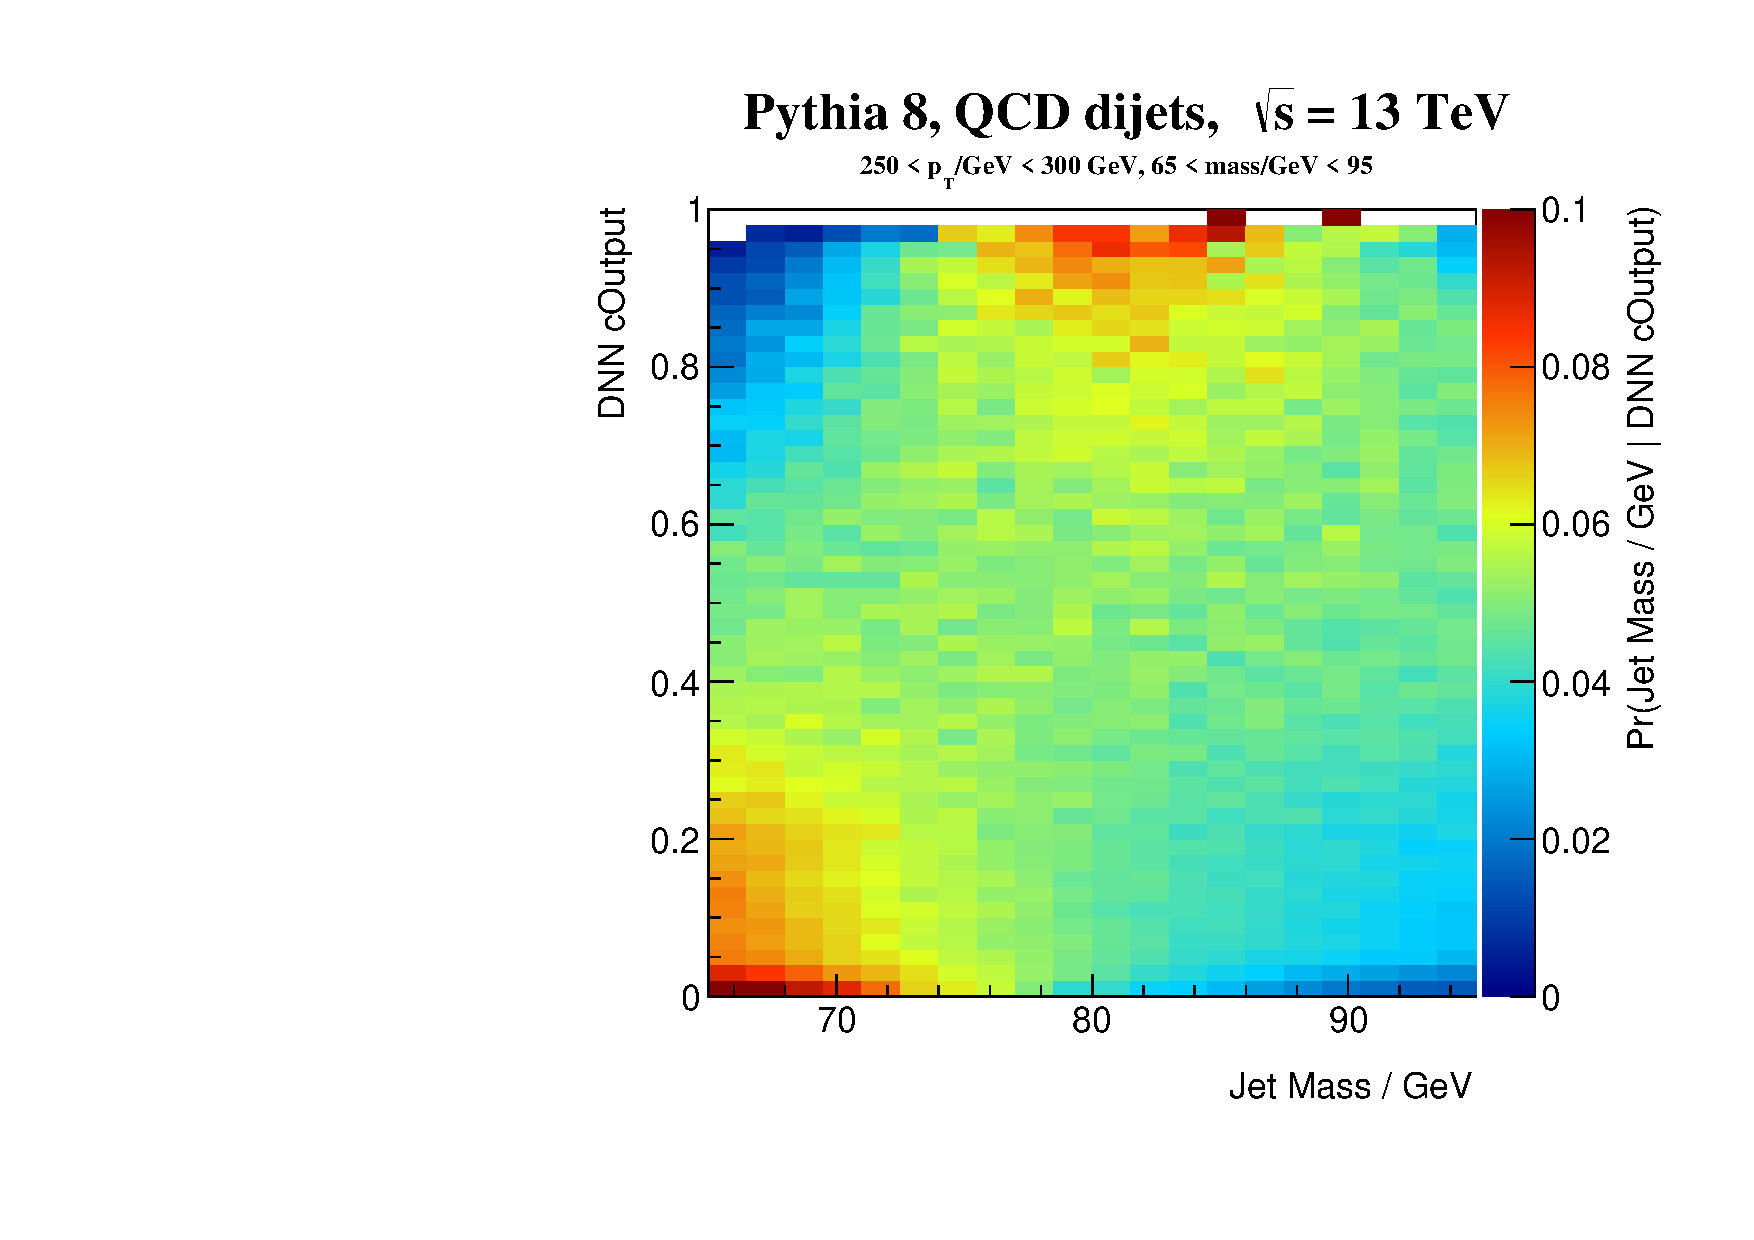
\includegraphics[width=0.45\textwidth]{figures/mass_convnet_back_norm_invert.pdf} 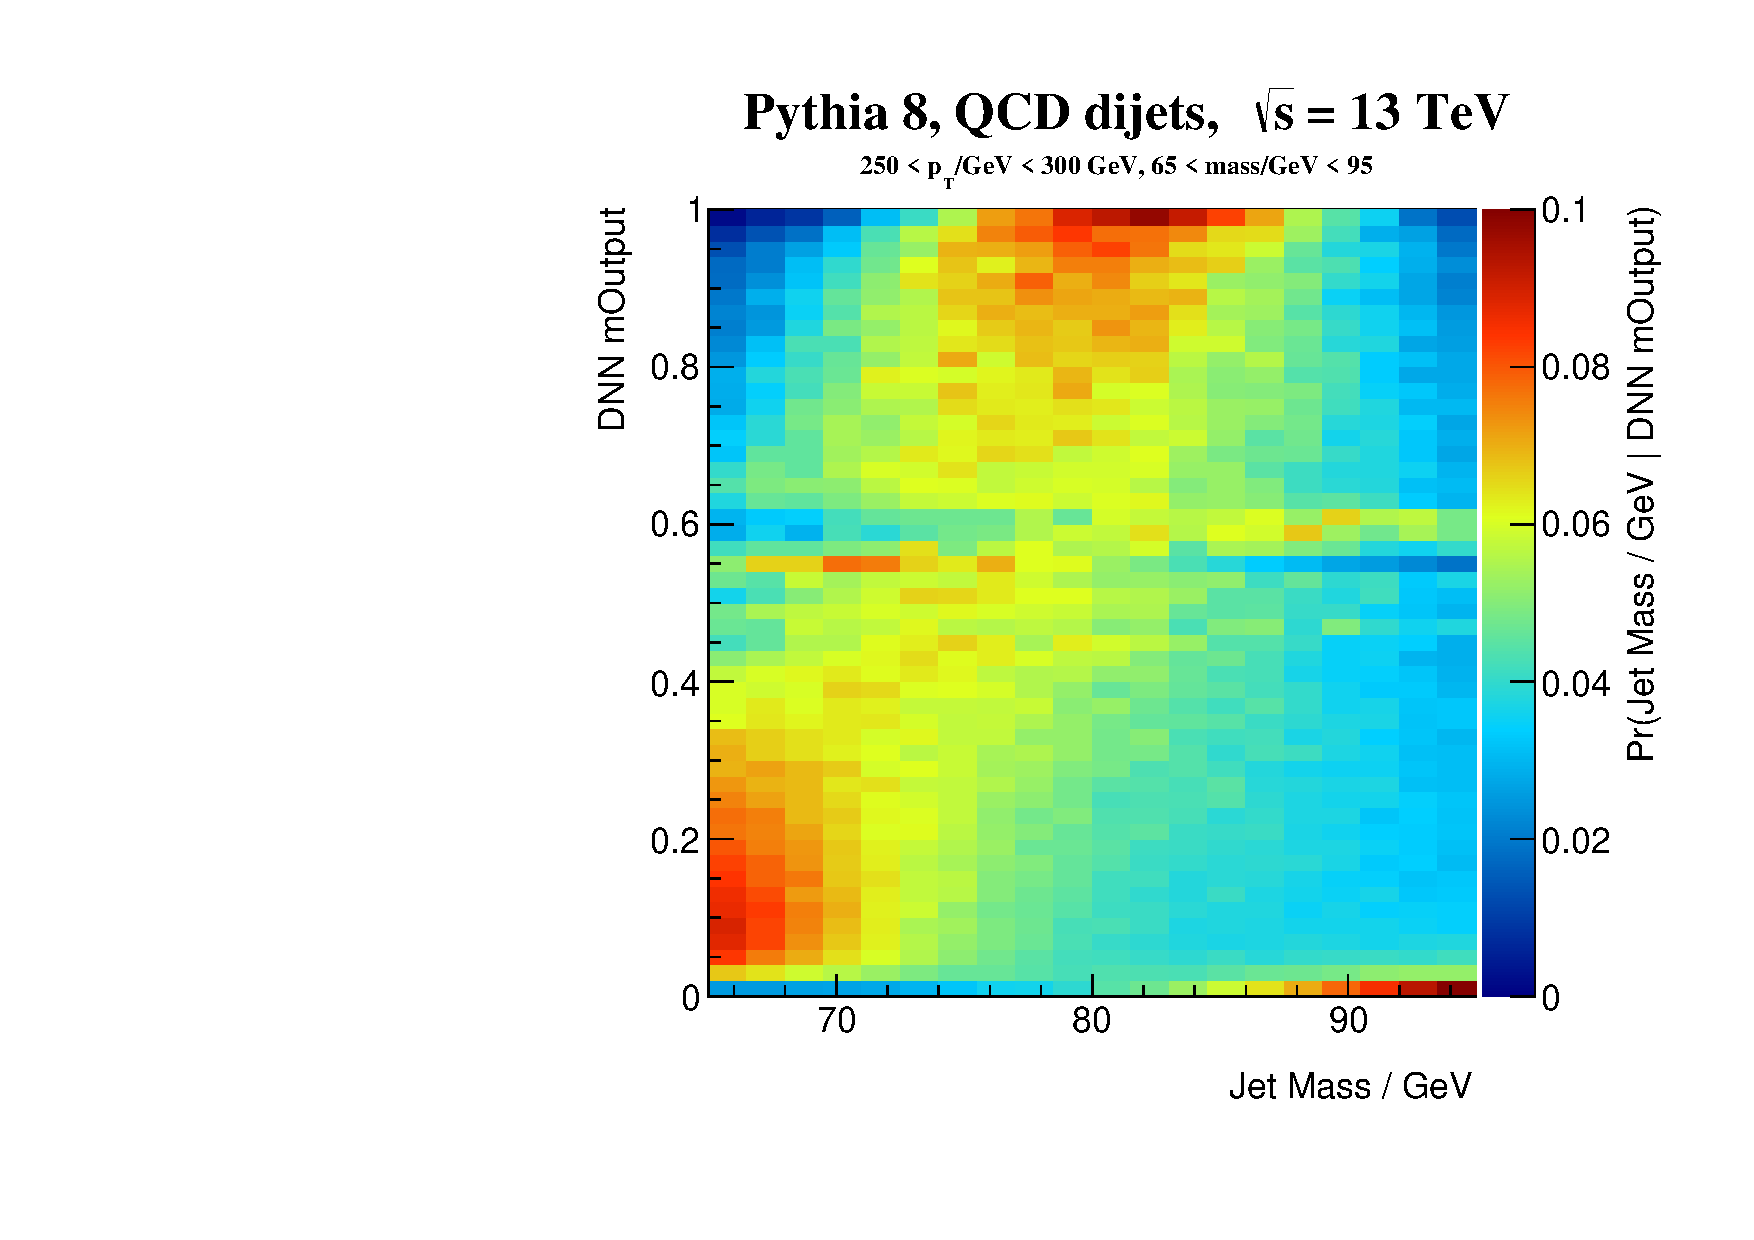
\includegraphics[width=0.45\textwidth]{figures/mass_maxout_back_norm_invert.pdf}
      }
      \\
      \subfloat[Sculpted QCD mass distribution\label{fig:sculptedmass}]
      {
        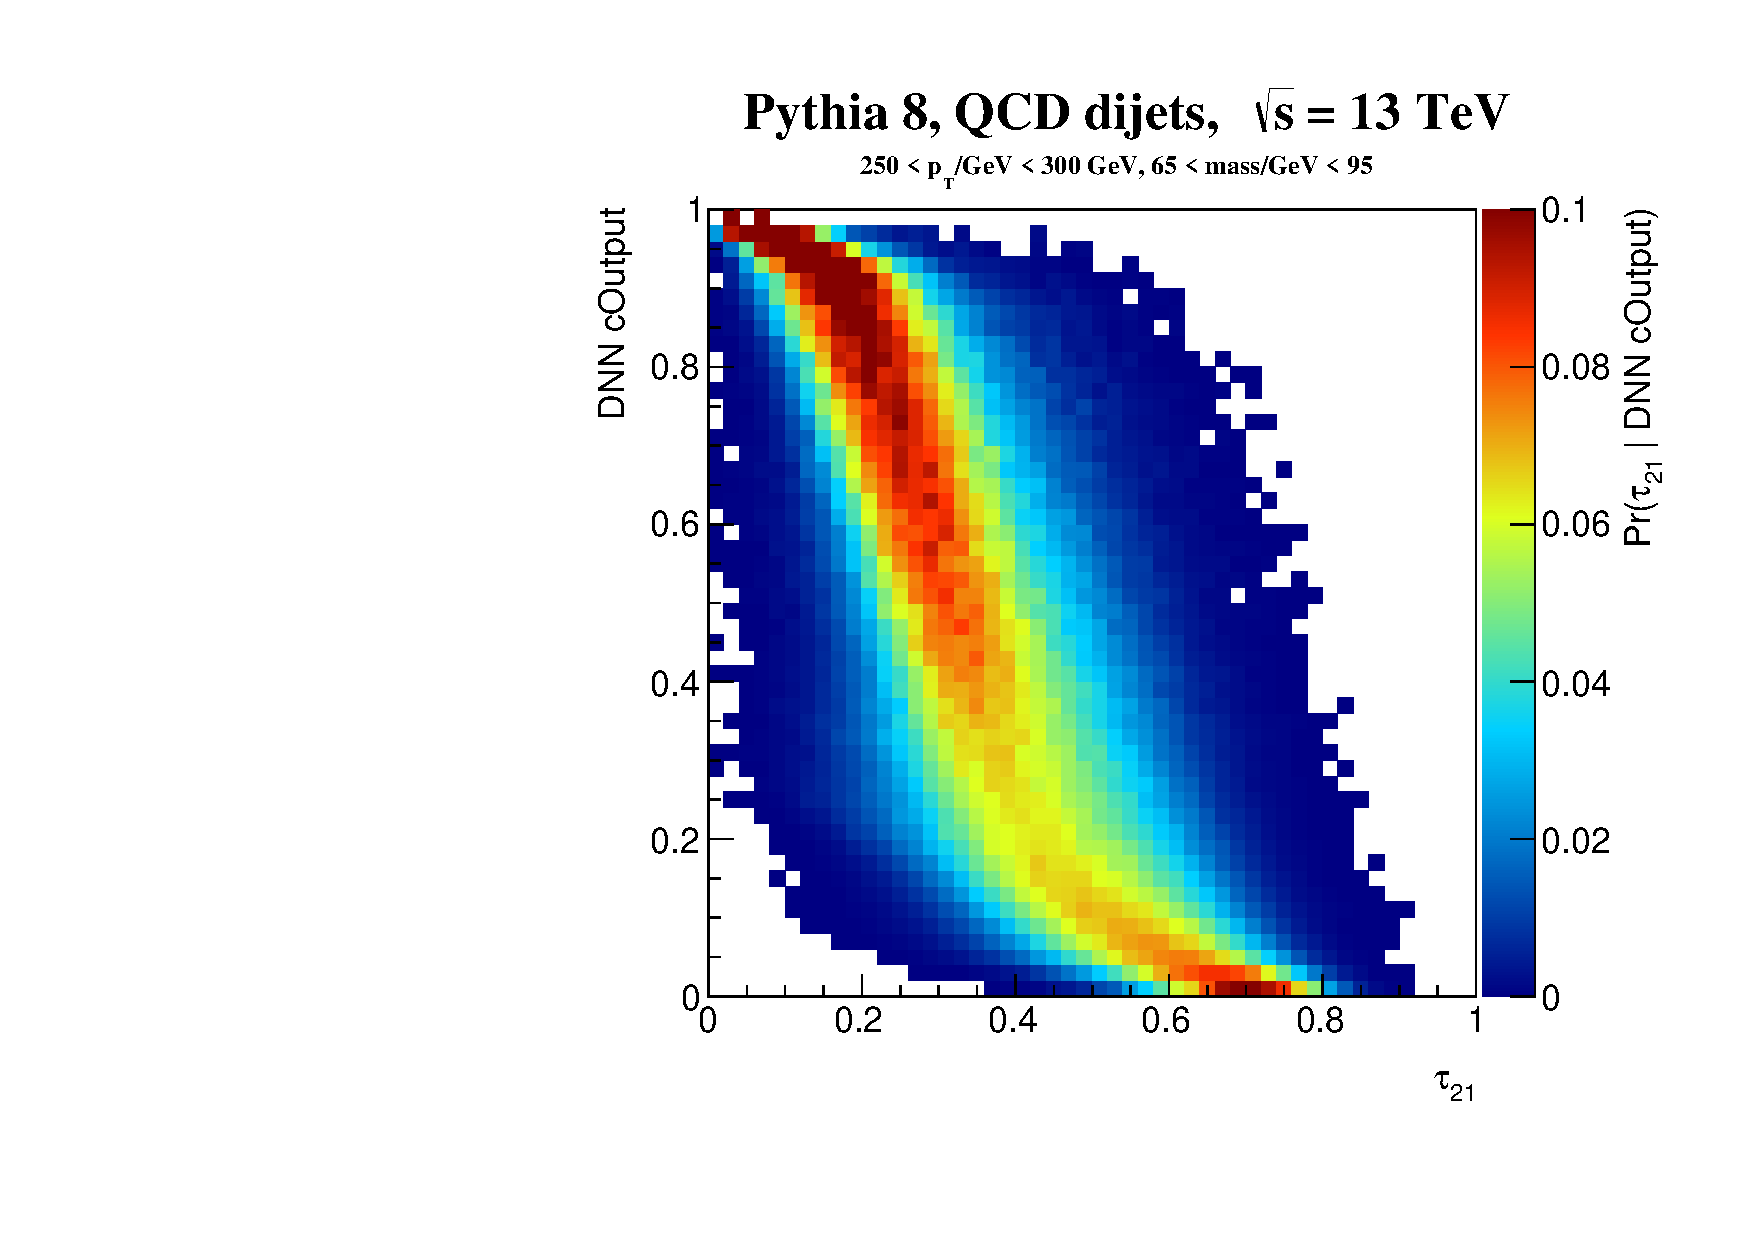
\includegraphics[width=0.45\textwidth]{figures/tau21_convnet_back_norm_invert.pdf} 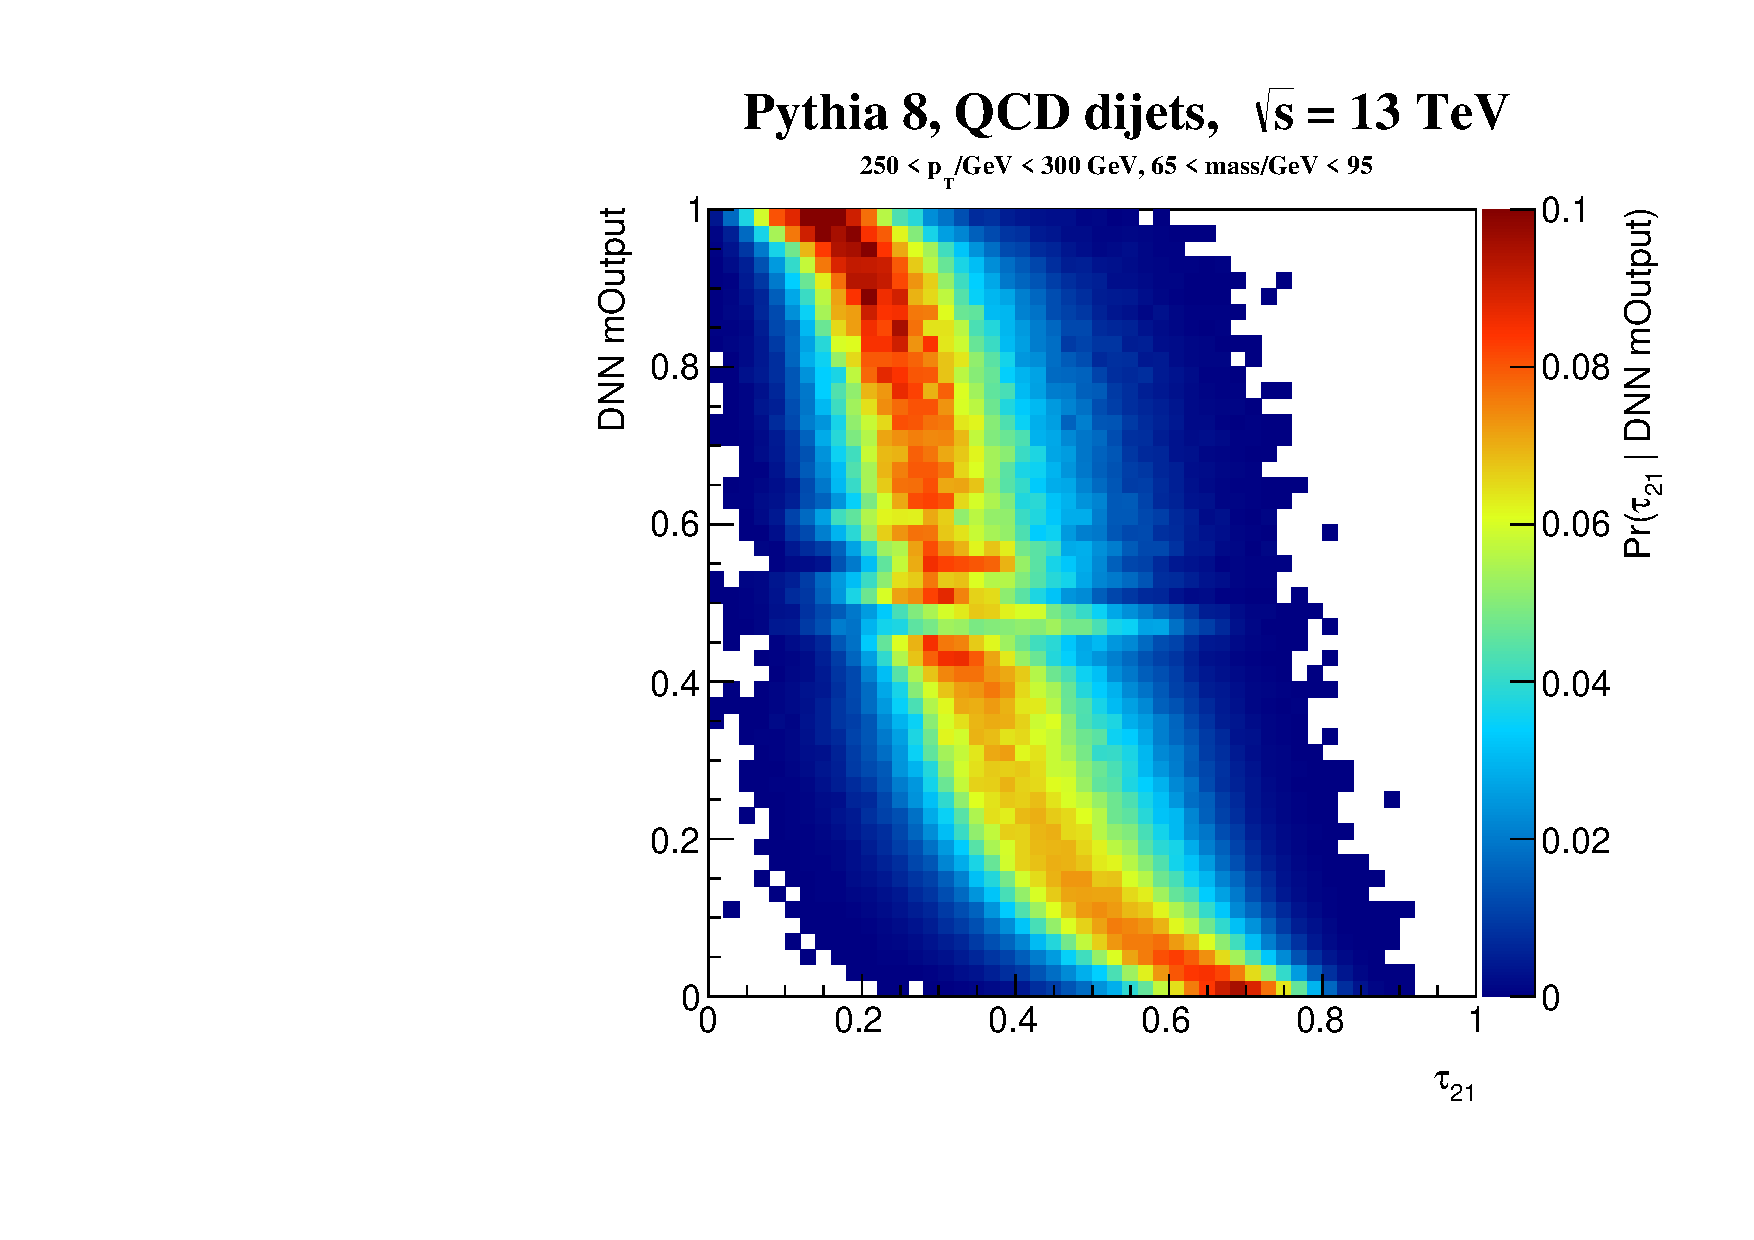
\includegraphics[width=0.45\textwidth]{figures/tau21_maxout_back_norm_invert.pdf}
      }

      \caption{Sculpted QCD distributions}
      \label{fig:qcdsculpt}

    \end{center}
\end{figure}

\begin{figure}[bt]
  \begin{center}
  
      \subfloat[Average $W'\rightarrow WZ$ image \label{subfig:sig_window}]{
        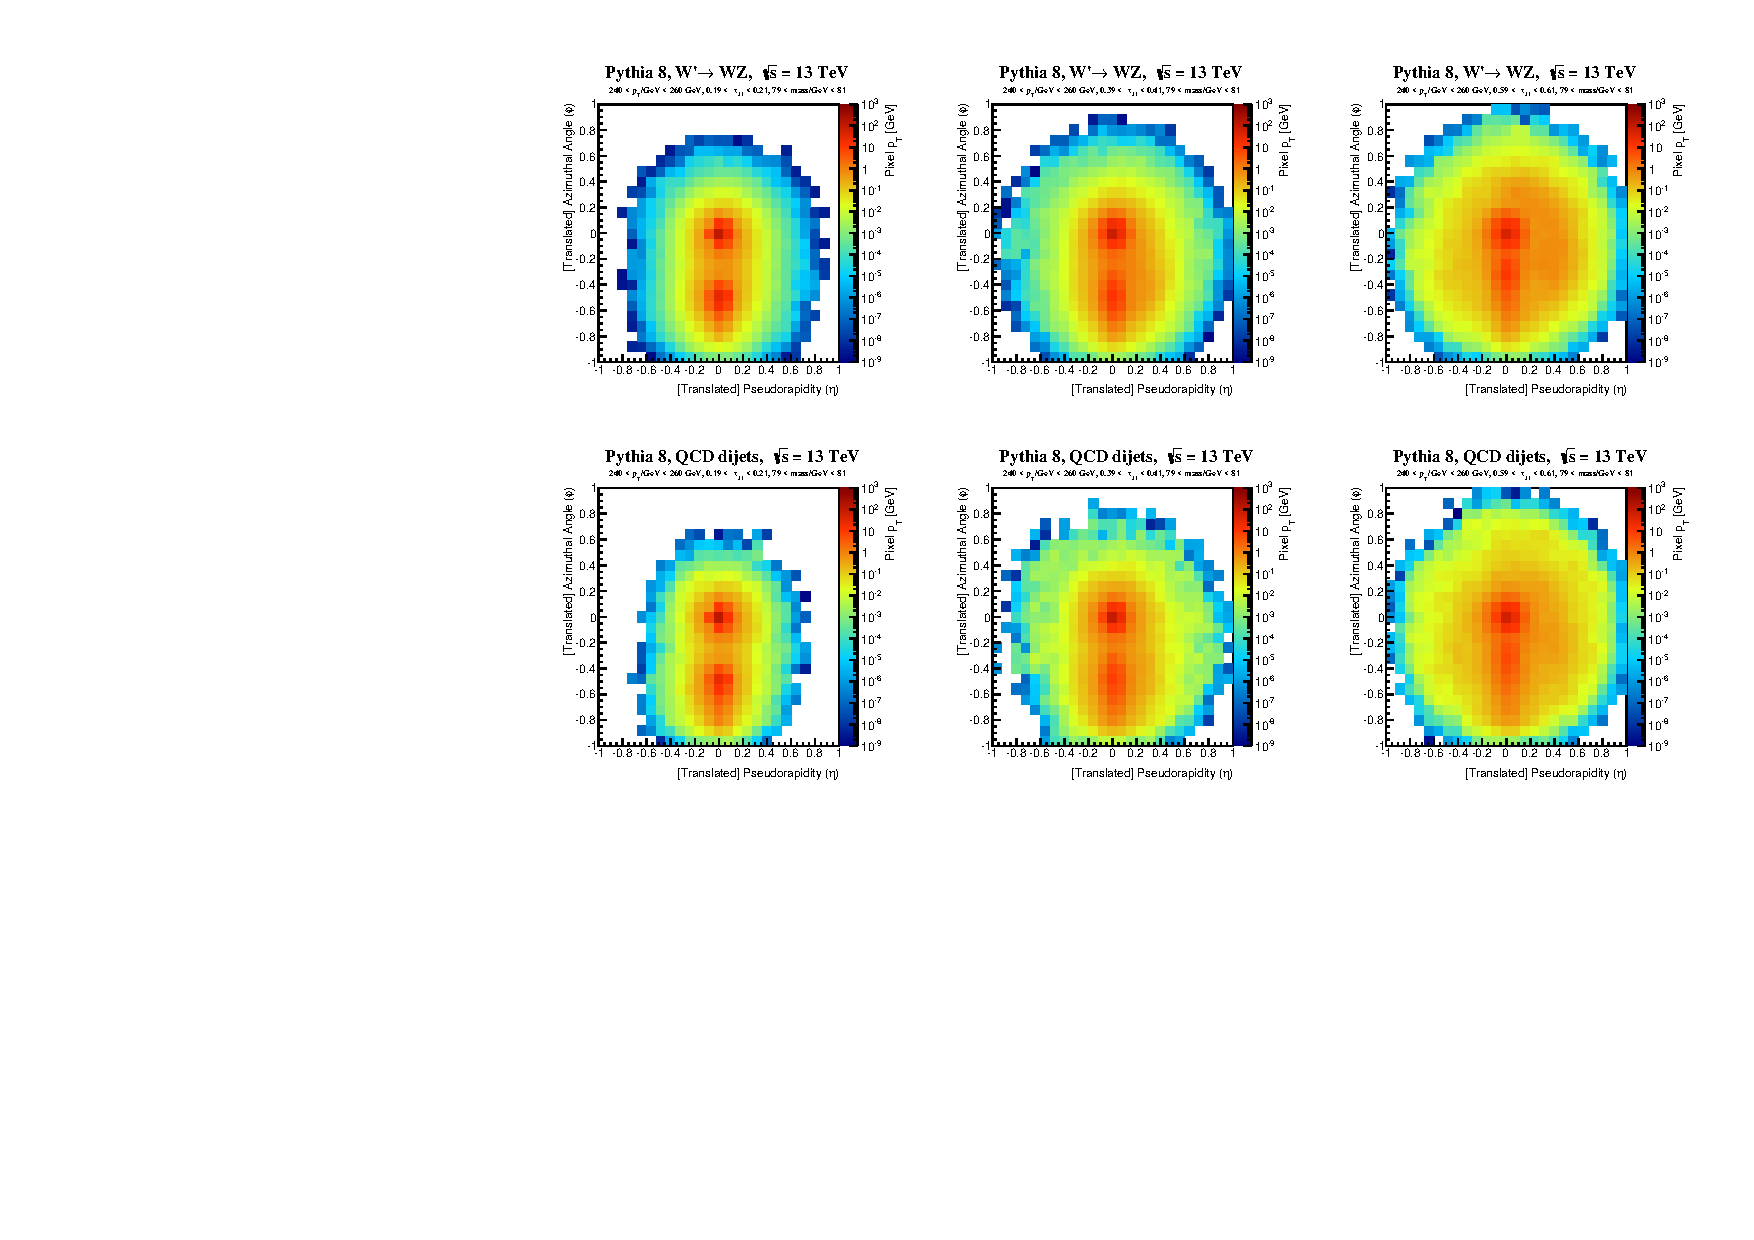
\includegraphics[width=0.99\textwidth]{figures/averages_fixed_nonorm.pdf}
      } \\
      \subfloat[Average image difference \label{subfig:windowdiff}]{
        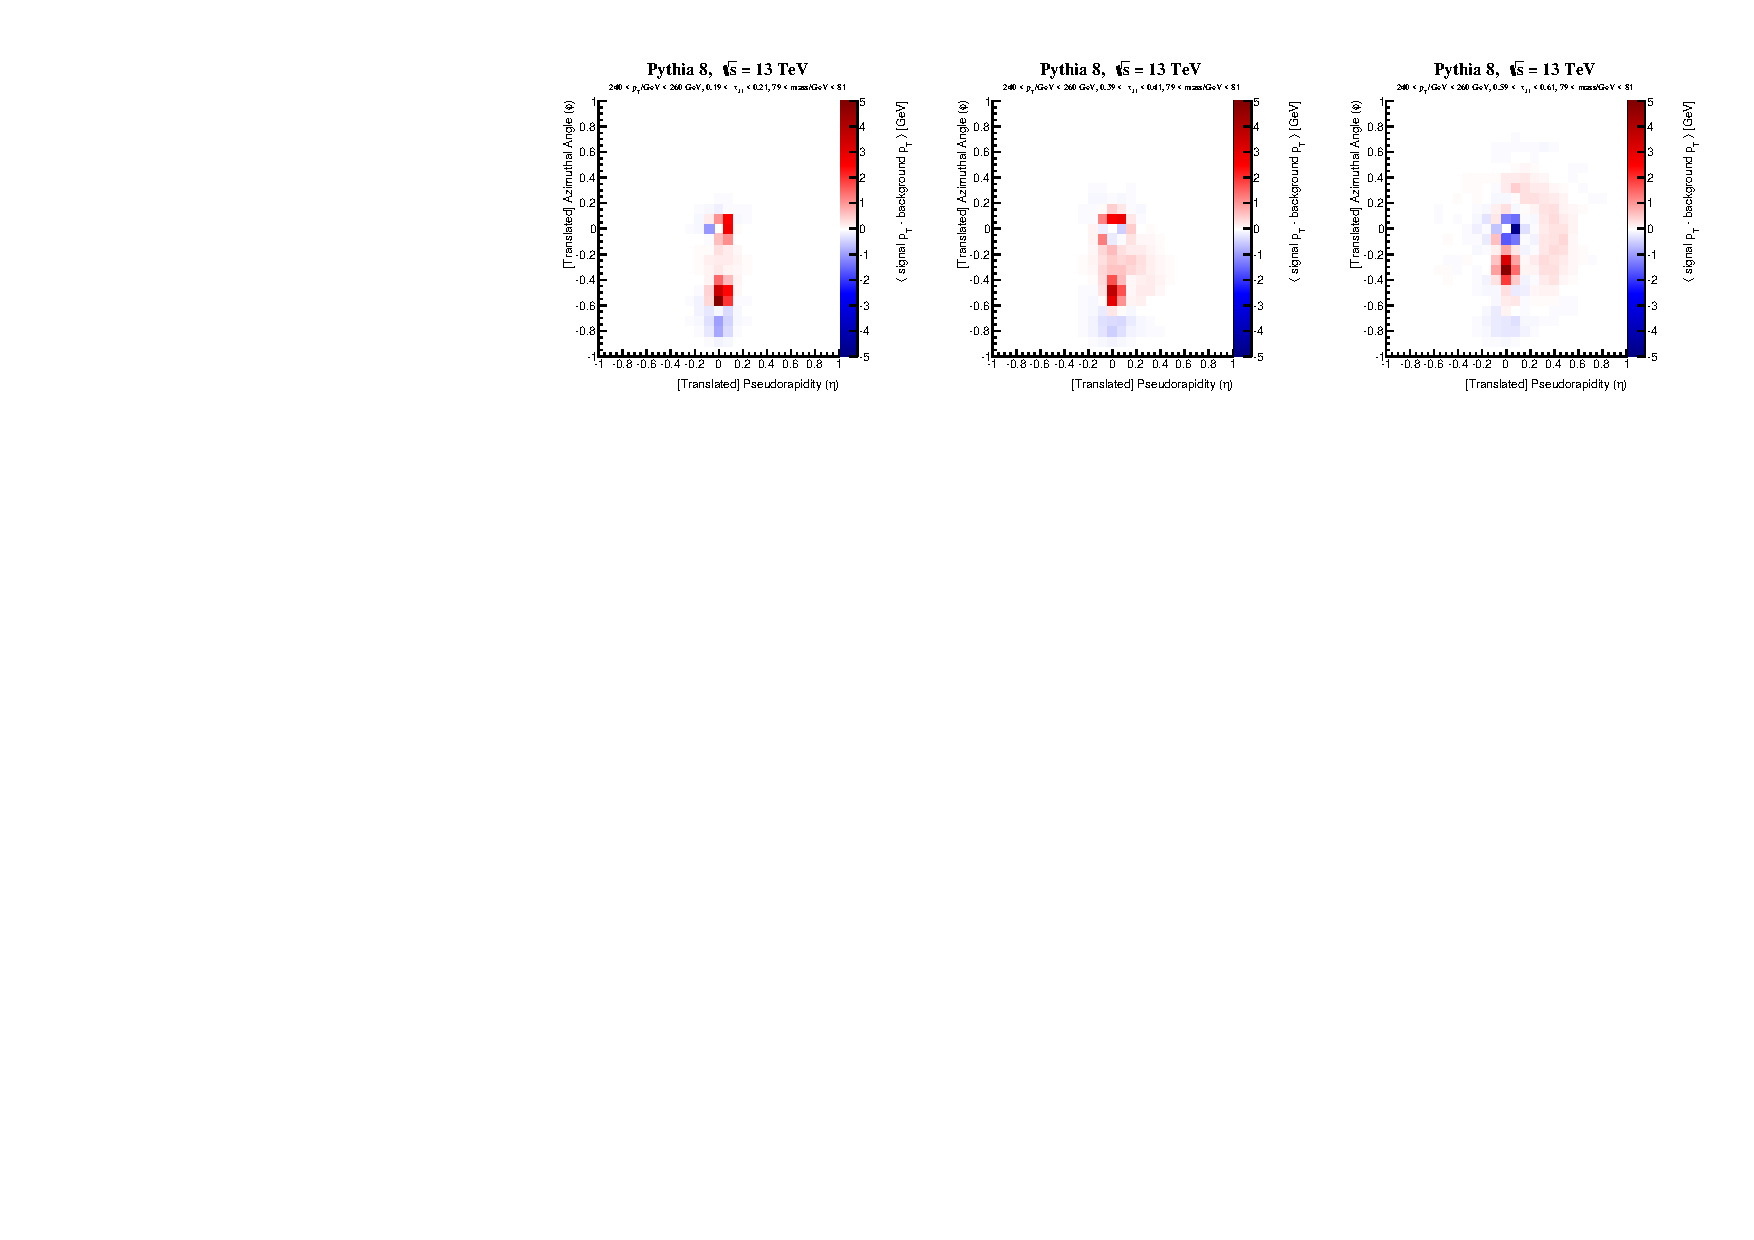
\includegraphics[width=0.99\textwidth]{figures/difference_fixed_nonorm.pdf}
      }
      \caption{
        $W'\rightarrow WZ$ (left) and QCD (right) average jet-images, and Signal - Background image difference (bottom)
        \label{fig:meanImagesWindow} 
      }
    \end{center}
\end{figure}  

In Figure~\ref{subfig:filters}, we show the (11$\times$11) convolutional filters learned by our network. To mimic the operation in the first layer of the network, we can convolve each filter with an average jet image to get an understanding of what features the network learns at the first layer. 

More formally, let $J_s=\frac{1}{n}\sum_{i:i\text{ is signal}} J^{(i)}$ and $J_b=\frac{1}{n}\sum_{i:i\text{ is background}}J^{(i)}$ represent the average signal and background jet over a sample, where $J^{(i)}$ is the $i$th jet image. In addition, we can select a filter $w_i\in\mathbb{R}^{11\times11}$ from the first convolutional layer.

We then examine the differences in the post convolution layer. We take 

\begin{equation}
  J_s \ast w_i - J_b \ast w_i, \forall i,
\end{equation}

where $\ast$ is the standard convolution operator. We arrange these new ``convolved images'' in a grid, and show in red regions where signal has a stronger representation, and in blue where background has a stronger representation. In Figure~\ref{subfig:convolvedfilters}, we show the convolved differences described above, where each $(i, j)$ image is the representation under the $(i, j)$ convolutional filter. We note the existence of interesting patterns around the regions where the leading and subleading subjets are expected to be. We also draw attention to the fact that there is a large diversity in the the convolved representations, indicating that the DNN is able to learn and pick up on multiple features that are descriptive.



\subsubsection{Physics in Deep Representations} % (fold)
\label{ssub:physics_in_deep_representations}

To get a tangible and more intuitive understanding of what jet structures a DNN learns, we construct the following. Let $y$ be the DNN output, and consider every pixel $p_ij$ in transformed $(\eta, \phi)$ space. We the construct an image where each pixel $(i, j)$ is $\rho_{p_{ij}, y}$, the Pearson Correlation Coefficient of that pixels energy deposition with the final DNN output. In Figure~\ref{fig:corr}, we construct this image, and can see interesting structure in the subleading subjet region as well as asymmetric scattering patterns around the leading subjet.




\begin{figure}[!htbp]
  \centering
  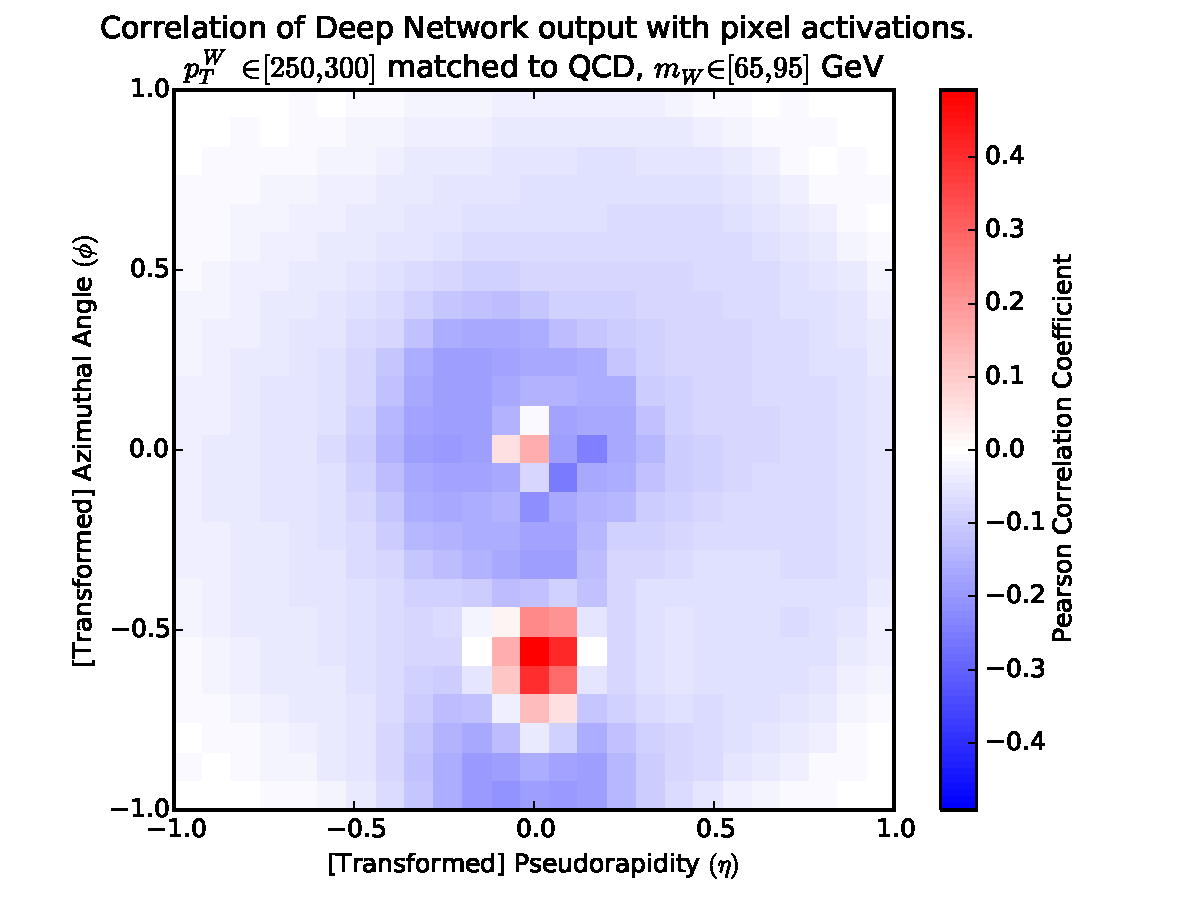
\includegraphics[width=0.95\textwidth]{figures/pixel-activations-corr.pdf}
  \caption{Per-pixel linear correlation with DNN output}
  \label{fig:corr}
\end{figure}

